% Draft Version 1 - Date 16/06/2020
% Draft Version 2 - Date 06/08/2020
% Draft Version 3 - Date 27/08/2020
% Draft Version 4 - Date 14/12/2020
\chapter[\titleres]{\titleres\footnote{Sections \ref{res-random} and \ref{res-fem} of this chapter are adapted from the final sections of the paper "N. G. Kilingar, K. Ehab Moustafa Kamel, B. Sonon, T. J. Massart, and L. Noels.	\textit{Computational generation of open foam representative volume elements with morphological control using distance fields.} European Journal of Mechanics - A/Solids, page 103847, September 2019."}}\label{chap-res}
\section{Introduction}
The macroscopic properties of open foam morphologies are highly affected by the internal micro-structure of the linkages made by the individual struts. Therefore, any representation of such micro-structures needs to be compared to the ``real'' micro-structure in question and such design tools need to be validated statistically. 

A lot of studies have been carried out to fit  models according to the material characterizations \cite{redenbachMicrostructureModelsCellular2009,vecchioAnglesLaguerreTessellation2014}. The statistical nature of these micro-structures implies that even though two structures obtained under same modeling conditions differ locally in their geometry, for relatively large samples, their statistical descriptors, such as the average pore size and pore size variations are the same. This allows establishing statistical relationships among some relevant features of these structures like variability of pore volume.

\red{A selective assessment of some of the morphological indicators of the foam, like the face-by-cell count, the edge-by-face count and the strut length distribution, is performed next based on the studies conducted in literature \cite{redenbachMicrostructureModelsCellular2009,vecchioImprovedModelsSolid2016,jungMicrostructuralCharacterisationExperimental2017,perrotPeriodicUnitCell2007}, showing that these properties are satisfactorily reproduced compared to the ones found in existing models generated by random Laguerre tessellations. A particular focus is set on properties related to open-cell aluminum foams with varying pore sizes. This assessment is used to demonstrate the flexibility  of the method, in comparison with ideal representations of such morphologies, to account for detailed micro-structural features such as strut shape variations, with a computational efficiency enabling the generation of a large number of volume elements of arbitrary size, at least when using the DN-RSA algorithm, for finite element simulations. A perfect and regular geometry would not be able to predict the plateau stress of the model\cite{wanExperimentalComputationalMicro2015}, and as such the geometrical intricacies, like waviness, is necessary. Such stochastic effects are naturally present when using DN-RSA algorithm to extract the morphologies and an assessment of the morphological indicators enables the user to understand the scope of application of the generated morphologies.}

Metal foams offer a tripartite macroscopic stress-strain response\cite{heinzeExperimentalNumericalInvestigation2018}. It can be divided into a linear pseudo-elastic region where a majority of struts behave in an elastic manner, a plastic collapse stress region where the stress plateau is obtained due to the successive collapse of pores in the specimen, and a densification region with a steep increase in stress once all the pores collapse (see Figure \ref{fig-int-sample}).
The pseudo-plastic region consists of a small number of struts that undergo plastic deformation leading to a overall reduction in the global stiffness of the foam. The foam's strength can be characterized by the point at which the plastic collapse begins. In this plastic collapse region, the overall stress remains constant. Due to the introduction of differing grain sizes largely due to the choice of the manufacturing method to obtain open foam specimens, a general reduction in the stiffness of micro-structure of the specimens is observed when compared to the bulk material properties\cite{andrewsCompressiveTensileBehaviour1999,markakiEffectCellWall2001,zhouInvestigationMicrostructureStrength2002}. Using a photogrammatry based optimization of the individual pores of the open foam specimen, it is possible to extract the modified bulk material properties to be used in a finite element based behavior analysis of generated foam morphologies\cite{heinzeExperimentalNumericalInvestigation2018}.

In this Chapter, the DN-RSA algorithm developed in Chapter \ref{chap-of} is first used to generate open foam morphologies that can be then validated by comparing various identifiers like face-by-pore, edge-by-face and edge-length distributions among others. Ways to verify the morphology on the basis of the foam density and the extracted strut cross-section are presented along with discussion of the generation of targeted morphologies. A reconstructed geometry using DN-CT-SCAN algorithm based on the CT-scans of an open foam specimen is then analysed by comparing the respective geometrical indicators. Finally, the behavior of generated random RVEs as well as the reconstructed geometry is presented.

The Chapter is outlined as follows: In Section \ref{res-random} morphologies of random RVEs extracted through tessellations of random spherical packings using DN-RSA are quantified. Following this, the morphology variations are verified. In Section \ref{res-ct} a reconstructed morphology using DN-CT-SCAN algorithm based on the images taken from the CT-scans of an open foam specimen is studied based on the geometrical indicators. Section \ref{res-fem} presents the results of numerical simulations on the RVEs generated randomly as well as on the reconstructed geometry comparing the ability of the framework to reproduce real foam behaviors.


\section{Morphology Quantification of the resulting RVEs}\label{res-random}
In this section, we quantify some of the important morphological parameters of the RVEs generated based on the  DN-RSA. We  first look at the properties that are directly related to the packing generation, and subsequently compare the properties of the meshed RVEs after the implementation of tools that use distance functions to vary the strut morphology.

\subsection{Validation of the Laguerre parameters}

The quantification of the morphological parameters is a necessary step in order to compare the properties of the resulting RVE geometry with real samples. Studies have been conducted to fit Laguerre tessellations to foam micro-structures, where it was observed that properties like cell volume, surface area, mean width and number of facets per cell are sufficient to fit the models to real samples \cite{vecchioAnglesLaguerreTessellation2014}. In \cite{redenbachMicrostructureModelsCellular2009}, observations of Laguerre tessellations generated by random packing of spheres with lognormal and gamma distributed volumes have been presented for various coefficients of variation (CV, ratio of the standard deviation and the mean of the volume distribution of the initial sphere packing). These observations show that for lower values of CV ($ <0.5 $), the chosen volume distribution and the sphere packing do not have a significant effect on the models generated. Since the aim of the procedure is to be used in multi-scale simulations, and commercially available metallic foams tend to have low CV ($ <0.1 $) \cite{perrotPeriodicUnitCell2007}, the present contribution is limited to lognormal distributions. 

\subsubsection{Methodologies}

Two approaches can be envisioned to evaluate the parameters under scrutiny.
\begin{enumerate}
	\item A ``classical'' approach makes use of the triangulated surfaces extracted from the level sets by contouring. Generally this approach can be used once the final mesh is generated and gives accurate values even for coarse discretizations. Apart from being able to calculate volumes and surfaces, by using the slicing functions discussed in the previous sections, isolated tessellation volumes can be extracted and their face, edge and node data can be characterized.
	\item An ``implicit'' approach directly makes use of the functions already computed, mainly $ NN_k $, $ DN_k $, $ O_V $ and $ O_P $. It has to be pointed out that the precision and accuracy of the results obtained in this approach largely depend on the size of the discrete grid used for the evaluation of these functions. Parameters that depend on the tessellation, like face-by-cell count and edge-by-face count can be calculated by counting the number of direct neighbors stored in the $ NN_k $ functions. The tessellation volumes and overall foam/coating volumes can be calculated by counting grid points with relevant values of the level set functions, and dividing the obtained number by the total number of grid points.
\end{enumerate}

An alternative way to quantify the morphology externally consists of using the convex hull approach with which, once the spheres packing is obtained, the tessellations can be simulated by constructing the convex hull of the centers of the spheres. The properties can then be extracted using QHull software package \cite{barberQuickhullAlgorithmConvex1996}, as detailed in \cite{redenbachMicrostructureModelsCellular2009} to study the properties of Laguerre tessellations. It should be noted here that the QHull package is extremely precise in modeling the tessellations. As a result, it is able to capture even the smallest faces and edges regardless of the discretization used. In the limit of a vanishing discretization size, this should also be the case for the ``implicit'' approach. However, in practice, with finite discretization grids, situations will arise in which two very close edges (or nodes) will be seen as a single one, shared by 4 or more faces (or 5 or more edges). Also, the geometries extracted from the ``classical'' approach will have already incorporated a finite edge thickness, resulting in further reduction of the number of faces per cell. 

\subsubsection{Number of faces per cell and number of edges per face}
Figure \ref{RSA_facecount} shows a comparison between various approaches to compute the number of faces per cell for an RVE constructed using free or non-constrained boundary conditions. Out of the 750 inclusions initially generated, only 400 remain inside the domain after minus sampling operation as discussed in Section \ref{text-minus}. The effect of refining the discretization grid for the function evaluations can be noticed in the increase in the mean number of faces captured using the ``implicit'' approach, with the curve shifting towards the data obtained from the QHull package as the number of grid points increases. It is also interesting to note that the ``classical'' method captures a lower number of faces per cell as explained before. Similarly, Figure \ref{RSA_edgecount} compares the effect of the different approaches for calculating the number of edges per face. As a value for comparison for these quantities, the mean number of faces per cell values ranges from 12 to 14 for a mono-dispersed 
%a table here c_1 c_2 ppi and others.
open foam (with very low CV), as analyzed by CT-scans according to various works that can be found in literature \cite{monnereauTopologySlightlyPolydisperse2001}. Similarly, the number of edges per face ranges between 5 and 5.5. Figure \ref{NF_CV} illustrates the effect of a variation of CV on two sample properties, i.e. the number of faces per cell and the coefficient of variation of the volumes of the resulting cells of the tessellation in comparison with that of the initial packing sphere volumes. These values are in sync with the values that were obtained in \cite{redenbachMicrostructureModelsCellular2009}.

\begin{figure}
	\centering
		\begin{subfigure}[b]{0.45\textwidth}
			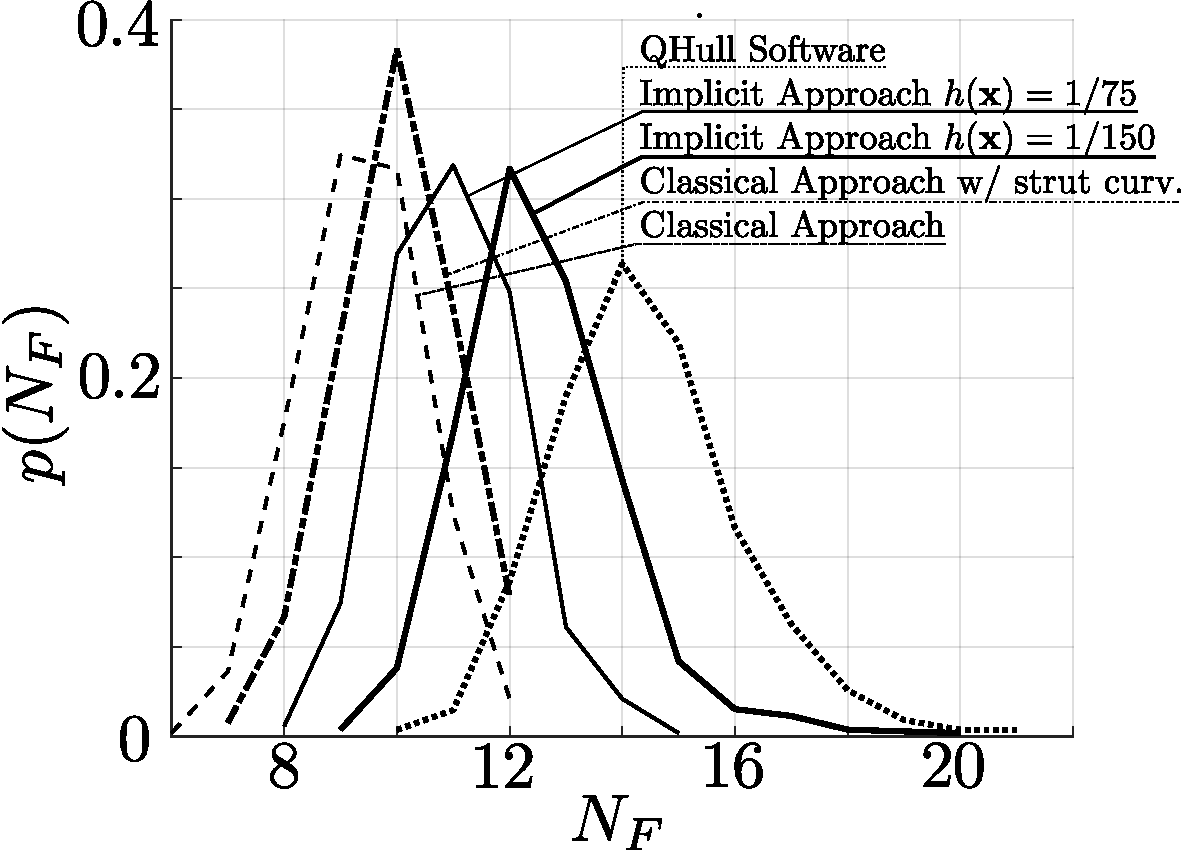
\includegraphics[width=\textwidth]{RSA_facecount_1}
			\caption{}\label{RSA_facecount}
		\end{subfigure}
		\begin{subfigure}[b]{0.45\textwidth}
			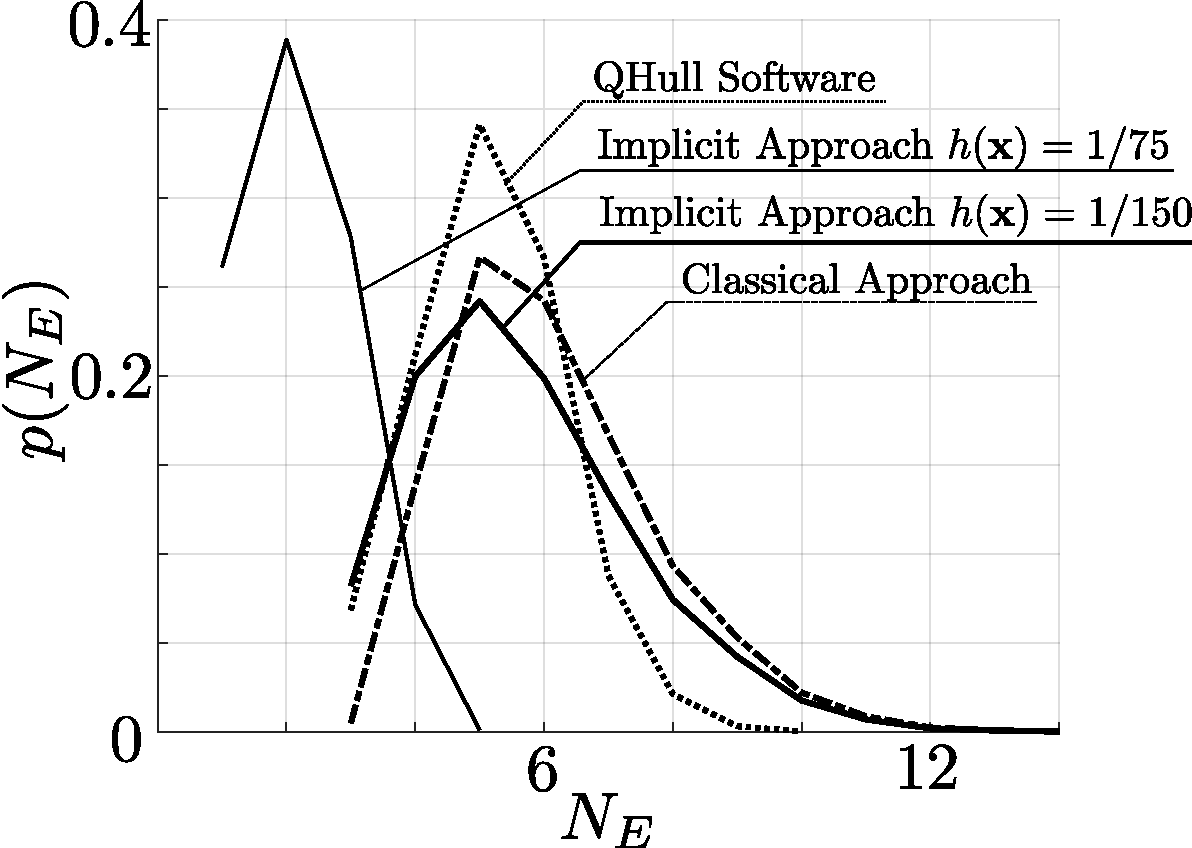
\includegraphics[width=\textwidth]{RSA_edgecount_1}
			\caption{}\label{RSA_edgecount}
		\end{subfigure}
	\caption{(a) Comparison of the occurrence of the number of faces per cell using various approaches for the same RVE obtained using DN-RSA algorithm with free boundary. (b) Comparison of the occurrence of the number of edges per face using various approaches for another RVE with free boundary. A sphere packing of 750 spheres has been generated with CV $ = 0.07 $.}
\end{figure}

\begin{figure}
	\centering
	\begin{subfigure}[b]{0.45\textwidth}
		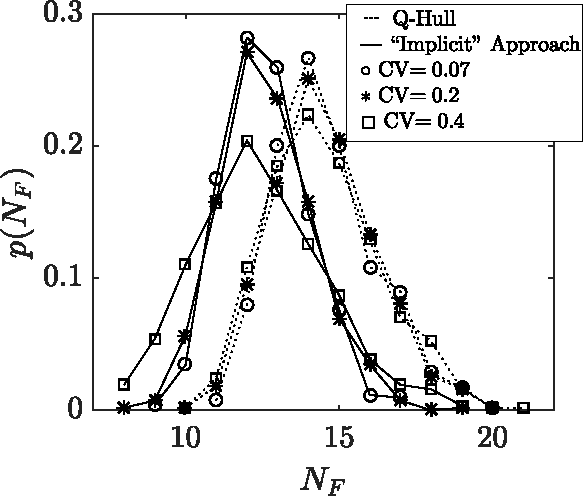
\includegraphics[width=\textwidth]{FPC}
		\caption{}
	\end{subfigure}
	\begin{subfigure}[b]{0.45\textwidth}
		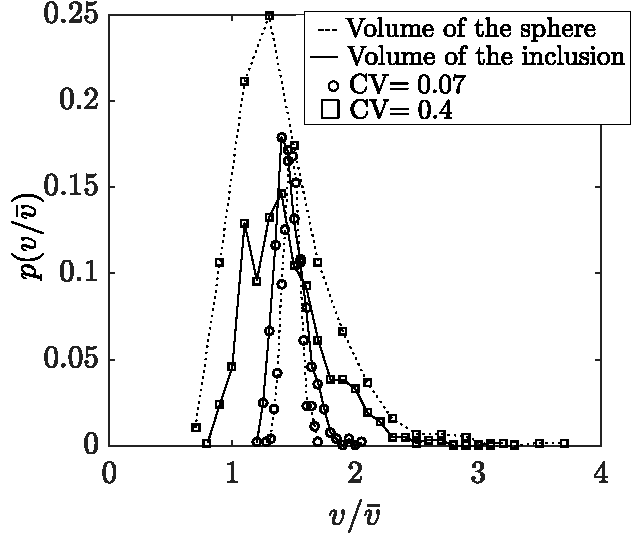
\includegraphics[width=\textwidth]{RAD}
		\caption{}
	\end{subfigure}
	\caption{(a) Variation of number of faces per cell with change in CV for the RVE obtaied using DN-RSA algorithm; (b) Comparison between the normalized volumes of the spheres in the initial packing and the normalized volumes of the resulting inclusions with variations in CV.}\label{NF_CV}
\end{figure}

%\hl{*May not be necessary as the studies have proven the following to be inconsequential.} 
%\textcolor{red}{Dihedral and interior angles (as defined in \cite{vecchioAnglesLaguerreTessellation2014}) also depend on the tessellation and can be extracted using the ``implicit" approach with the help of $ NN_k $ and $ O_V $ \cite{sononAdvancedApproachGeneration2015}. However, we will not take these into consideration as studies have shown that by taking into consideration the cell volume, mean width of the cell and the number of facets per cell, model fit of random Laguerre tessellations can be achieved with foam samples \cite{vecchioAnglesLaguerreTessellation2014}.
%}
\subsubsection{Edge length distribution}
The  ``implicit" approach provides a very straightforward approach to compute the edge length distribution of an RVE. By making use of operator (\ref{variation1}), a distribution of the edge length can indeed be obtained. In the ``classical" approach based on triangulated surfaces, the introduction of a finite thickness for the struts results in very small faces and edges being absorbed and represented as very thick struts. This factor cannot be included in the ``implicit" approach directly. A relation graph between the cells, faces, edges and nodes can be built, and a comparison between the ``implicit" and ``classical" approaches based on this graph can help evaluating the exact number of struts in the generated RVE. 
%As can be seen from Figure \ref{RSA_edgelength}, the distribution of normalized edges extracted by ``implicit" approach follows a pattern similar to that extracted by QHull \cite{vecchioImprovedModelsSolid2016}. 
Many studies, like \cite{vanderburgLinearElasticProperties1997,kanaunMechanicalPropertiesOpen2006}, utilize structural beams with uniform cross-section to represent the struts in the RVE and introduce a control on the minimum strut length by collapsing struts shorter than a tolerance parameter to a single node, in order to decrease the computation time. This is not necessary when constructing RVEs using distance functions, as the struts are implicitly meshed based on the extracted isosurfaces before generating a volume mesh. The influence of relatively short struts is therefore expected to have almost no effect on the mechanical behavior of the unit cell. This technique is however helpful in getting a rough estimate of the strut length distribution. In general, the Q-Hull approach generates the data of the tessellations in the form of a list of polygons that form the faces of the individual cells, which can then be compared with the relation graph to identify such short struts and also the resultant closed faces. One can then merge all the nodes that are close to each other for these identified faces and obtain the data about an approximate strut length distribution. Figure \ref{RSA_edgelength} illustrates the variation of the normalized edge lengths with respect to changes in CV as computed by Q-Hull, which shows trends similar to those found in \cite{vecchioImprovedModelsSolid2016} for Laguerre tessellations. The distributions become more Gaussian when comparing the lengths with the relation graph in which all the small edges and faces are absorbed by the implementation of a thickness parameter ($ t $, in these simulations, is chosen such that the ratio between the pore diameter and the strut thickness is approximately $ 6:1 $). 

\red{Having said this, it is possible to locate the common nodes using the corresponding level sets and implement structural beam elements to replace the level-set derived geometry completely. This could be helpful in obtaining a quicker, coarser geometry, but could lead to accumulation of material at nodes due to the overlap of multiple struts at the junctions.}
%Page 11 van der burg

\subsubsection{Conclusions on the statistical distribution of RVE properties}
The study of the aforementioned properties of the tessellations developed using distance functions of packings generated by DN-RSA shows that they sufficiently match the ones developed by existing tools in literature. These studies have also shown that, for sufficiently low CV values, the models fit quite well with real samples, i.e. the randomness generated by using Laguerre tessellations matched the natural randomness of open foams with mono-dispersed inclusions primarily considered in industrial applications. 

To model such foam samples, it is sufficient to consider a large number of closely packed spheres so that in a non-periodic RVE, even after the use of minus-sampling, as explained in Section \ref{text-minus}, 
% Remarks
there will be a sufficient number of inclusions that will allow properly reproducing the randomness of the foam sample. Table \ref{tab_minus_sampling} analyses the relation between the average size of the inclusions, represented here in terms of the number of inclusions in the domain, and the maximum permissible unit length for minus sampling. It can be seen that with an increase in the number of inclusions in the RVE, more inclusions can be retained inside the reconstructed domain. However, it also means that non-periodic RVEs need to be larger than the periodic RVEs to compensate for the loss of the resulting domain due to minus sampling.


%Even though it is possible to generate periodic packing with DN-RSA, the generation of a periodic RVE of a foam is still under development as the triangulations after splitting of the \textit{isosurfaces} of the inclusions need to maintained periodic in nature as well as the effect periodicity has on the packing, and the RVE needs to be studied seperately. It is possible that with an RSA packing, the periodicity will leave no impact different than that in a non-periodic RVE due to the extra randomness the $ nnl $ variables introduce. In general, a periodic packing generation is quite slower compared to a non-periodic one.

\begin{figure}
	\centering
	\begin{subfigure}[b]{0.45\textwidth}
		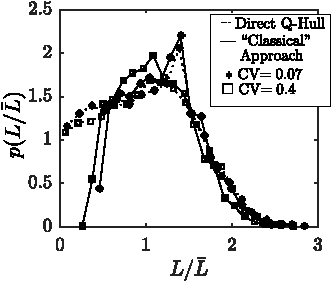
\includegraphics[width=\textwidth]{LENGTH}
	\end{subfigure}

	\caption{Normalized edge length distribution of an RVE with free boundary.}\label{RSA_edgelength}
\end{figure}

\begin{table}
\small{
	\begin{center}
		\caption{Study of the effect of minus sampling on the number of inclusions that can be used for the extraction of an open cell foam RVE.}\label{tab_minus_sampling}
		\begin{tabularx}{\columnwidth}{X|X|X}
			\hline
			Total spheres in the initial packing  & Inclusions remaining after minus sampling & Maximum permissible unit length for minus sampling (\% of initial RVE length)\\[0.5ex]
			\hline
			331 & 122 & 70\%\\[1ex]
			438 & 172 & 74\%\\[1ex]
			483 & 229 & 78\%\\[1ex]
			564 & 277 & 80\%\\[1ex]
			690 & 331 & 81\%\\[1ex]
			751 & 402 & 82\%\\[1ex]
			\hline
		\end{tabularx}
	\end{center}}
\end{table}

\subsection{Verification of morphology variation}
\subsubsection{Foam density}
As in the previous section, the morphological variations obtained by the ``post-processing", or the extraction of the RVE geometry through the combination of distance functions can also be investigated using both the ``implicit" and the ``classical" approaches. For a sufficiently mono-dispersed foam, the developed model can mimic the changes due to the variations in ppi by introducing variations in the strut morphology without the need to build models with a large number of inclusions to achieve the same results. As can be seen in \cite{jungMicrostructuralCharacterisationExperimental2017,perrotPeriodicUnitCell2007}, the strut cross-section changes from a plateau-border configuration to a circular shape as the ppi value increases. This can be explained by the solidification of the base PU foam before reaching equilibrium at lower ranges of the sample dimensions. This variation can also be seen in the excess accumulation of material at mid-section of the struts in higher ppi foam samples.

The density of the foam can be computed ``implicitly'' by counting the grid points with relevant values of the $ O_P $ function. In the ``classical'' approach this can be achieved by calculating the sum of the volumes of the tetrahedral elements in the RVE mesh. To achieve variations in the ppi value, and thus the density in an RVE with unit dimensions, the variations in the strut cross-section play an important role. Table \ref{tab_relden} shows that the difference in the computed densities between the two approaches remains rather small. Since the ``implicit" calculation can be implemented as a post-processing operation of DN-RSA without extracting the mesh, the relative density can be computed initially, and then adjusted using  the quantities that influence the strut cross-section variation and thickness to obtain an RVE with a ppi value close to the real samples. Figure \ref{density_t} compares the effect of a strut cross-section variation and of a changing thickness parameter on the overall porosity computed by the ``implicit'' approach.

Based on the manufacturer's description or on previous studies on foam samples using CT-scans, it is possible to build a link between the ppi values and the average cross-sectional area of the struts of the foam at mid-sections. Based on \cite{jangMicrostructureOpencellFoams2008,jungMicrostructuralCharacterisationExperimental2017,perrotPeriodicUnitCell2007}, the values of $ c_1 $ and $ c_2 $ in Eq. (\ref{strut1}) as well as the control on concavity, $ k_c $ in Eq. (\ref{concavity-eq}), can be assigned. These values have to be calculated on a case by case basis. However, a general database can be prepared, with variations in the values that depend on the manufacturing process used for the foam and the degree of inclusion volume dispersion. 

\begin{table}
\small{
	\begin{center}
		\caption{Comparison of relative density calculated by the two approaches for an RVE with free boundary. Density variations was achieved by modifying the variables influencing the strut cross-section.
	%			 with variations in $ t $, $ c_1 $, $ c_2 $ and $ k $ values.
}\label{tab_relden}
		\begin{tabularx}{\columnwidth}{c c c}
			\toprule
			``Classical" Approach & ``Implicit" Approach & Difference\\[0.5ex]
			\midrule
			0.0216 & 0.0205 & 5.09\%\\[1ex]
			0.0647 & 0.0586 & 9.42\%\\[1ex]
			0.0641 & 0.0614 & 4.21\%\\[1ex]
			0.0652 & 0.0604 & 7.36\%\\[1ex]
			\bottomrule
		\end{tabularx}
	\end{center}}
\end{table}
%\begin{figure}
%	\centering
%	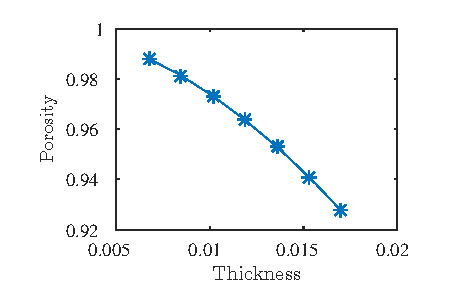
\includegraphics[]{density_t_plot}
%	\caption{Variation of porosity with changing $ t $ value in $ O_P $ function.}\label{density_t}
%\end{figure}

\begin{figure}
	\centering
	\begin{subfigure}[b]{0.5\textwidth}
		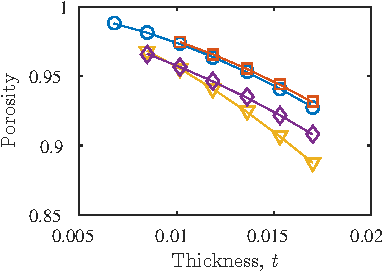
\includegraphics[width=\textwidth]{porosity_t_plot}
	\end{subfigure}
	\caption{Variation of the RVE porosity with strut thickness and cross-section variations in Eqs (\ref{strut1}) and (\ref{concavity-eq}); Legend - $ \circ $: $ c_1=20 $, $ \square $: $ c_1 = 60 $ denoting thinner strut cross-section at mid strut, $ \triangle $: $c_1 = 3$ denoting almost uniform cross-section, and $ \Diamond $: $ c_1 = 20 $, $ k_c=-0.5 $ with convexity in the strut cross-section.}\label{density_t}
\end{figure}

\subsubsection{Struts cross-section}
Individual sample struts can be analyzed using the ``implicit" approach, by identifying the four nearest inclusions of the struts, identifying the grid points of the strut by matching them with respective $ NN_k $ values and calculating the value of $ O_P $ at these grid points. Using the ``classical'' approach, the tetrahedra elements that form the struts can be identified due to their proximity to the grid points identified in the ``implicit" approach. The discretization grid however needs to be very small to have a good approximation of the analysis of a strut using the ``implicit" approach. It can also be used as a starting point to analyze the struts through the ``classical" approach.  
Figure \ref{strut_section} illustrates a strut extracted from an RVE and the variation of the cross-sections along the axis. It is to be noted that the ends of the struts are already a part of the node and thus the sections in these parts are not triangular anymore.  {This also ensures that material accumulation due to overlapping struts does not happen since the extracted surface is a direct result of the distance function.}  {Figure \ref{strut_section_variation} compares the variations in the concavity-convexity that can be obtained by varying the concavity parameter $ k_c $. 
%However, it has to be noted that using DN-RSA to obtain circular cross section is unnecessary as the extraction of sharp edges is an unnecessary process.
} 
The variation of the relative area along the axis of 5 sample struts extracted from an RVE is illustrated in Figure \ref{strut_section_plot} in which it can be seen that, when compared to the relative area variation of a strut taken from a real foam, the RVE mimics the strut cross-section faithfully.


%\begin{enumerate}
%	\item isosurface extraction by fft
%	\item surface intersection/boolean approaches on surface, resulting intersections, sharp edge remeshing
%	\item mesh refinement for the surfaces
%	\item tetgen based 3d
%	\item  FLOWCART  Surface intersection
%\end{enumerate}
%\subsection{Sharp edge refinement}
\begin{figure}
	\centering
	\begin{subfigure}[b]{0.45\textwidth}
		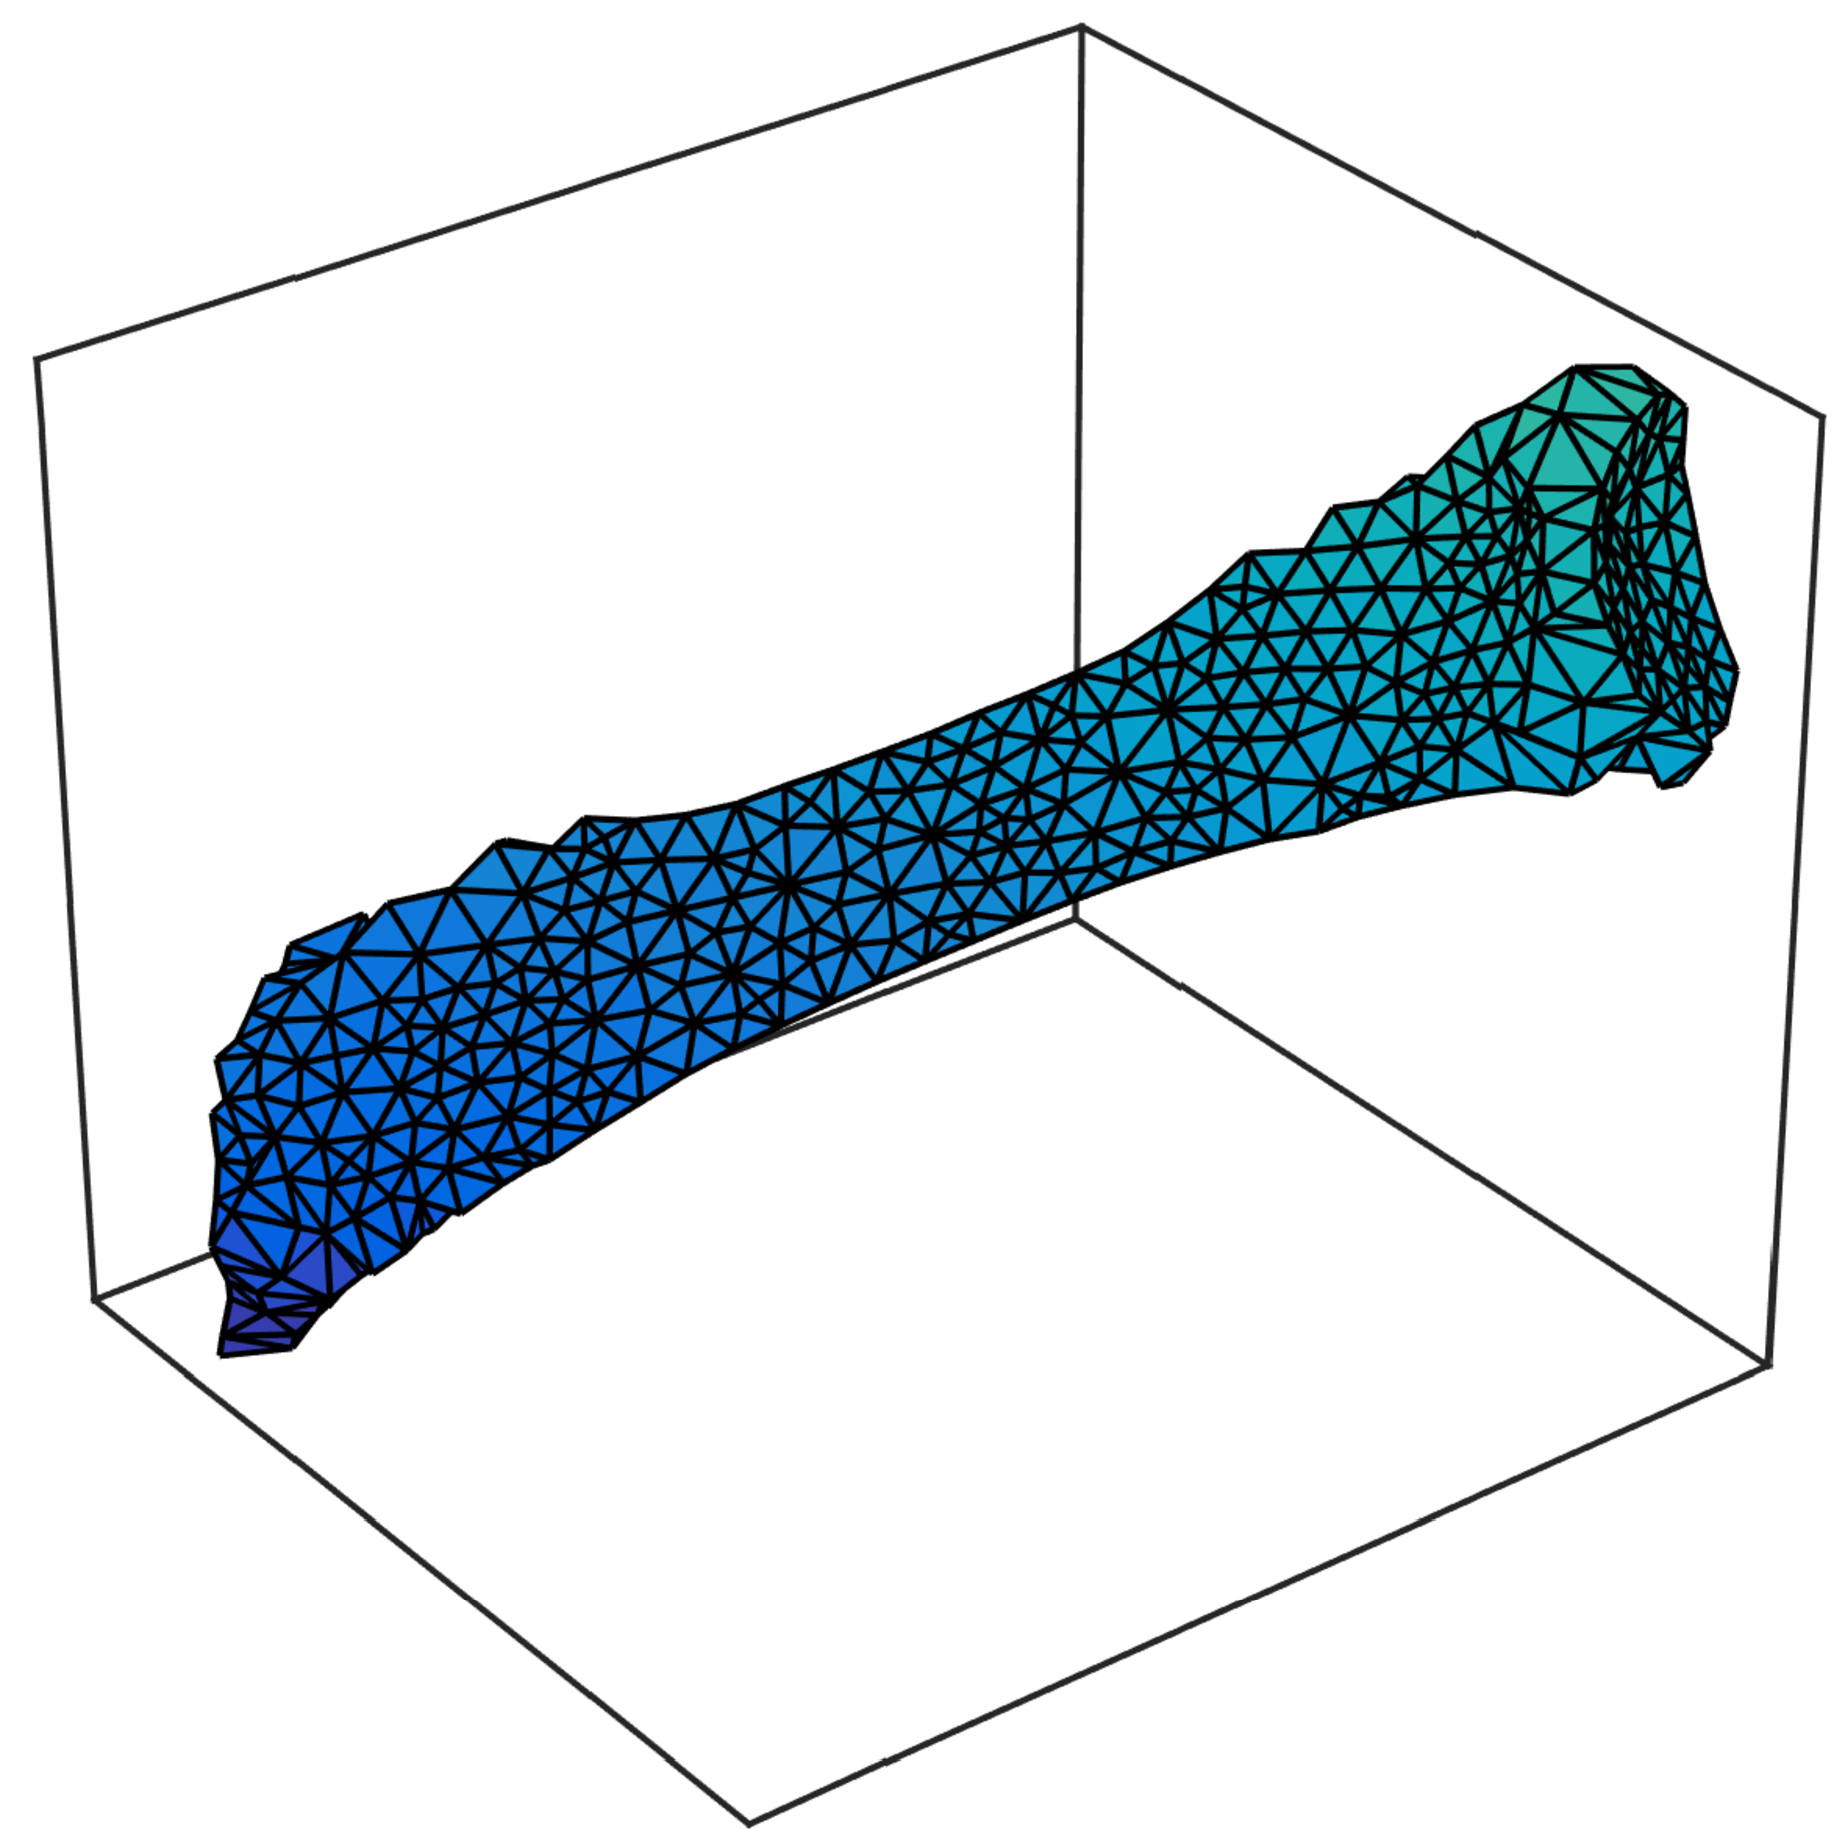
\includegraphics[width=\textwidth]{STRUT_SINGLE}
	\end{subfigure}
	\begin{subfigure}[b]{0.45\textwidth}
		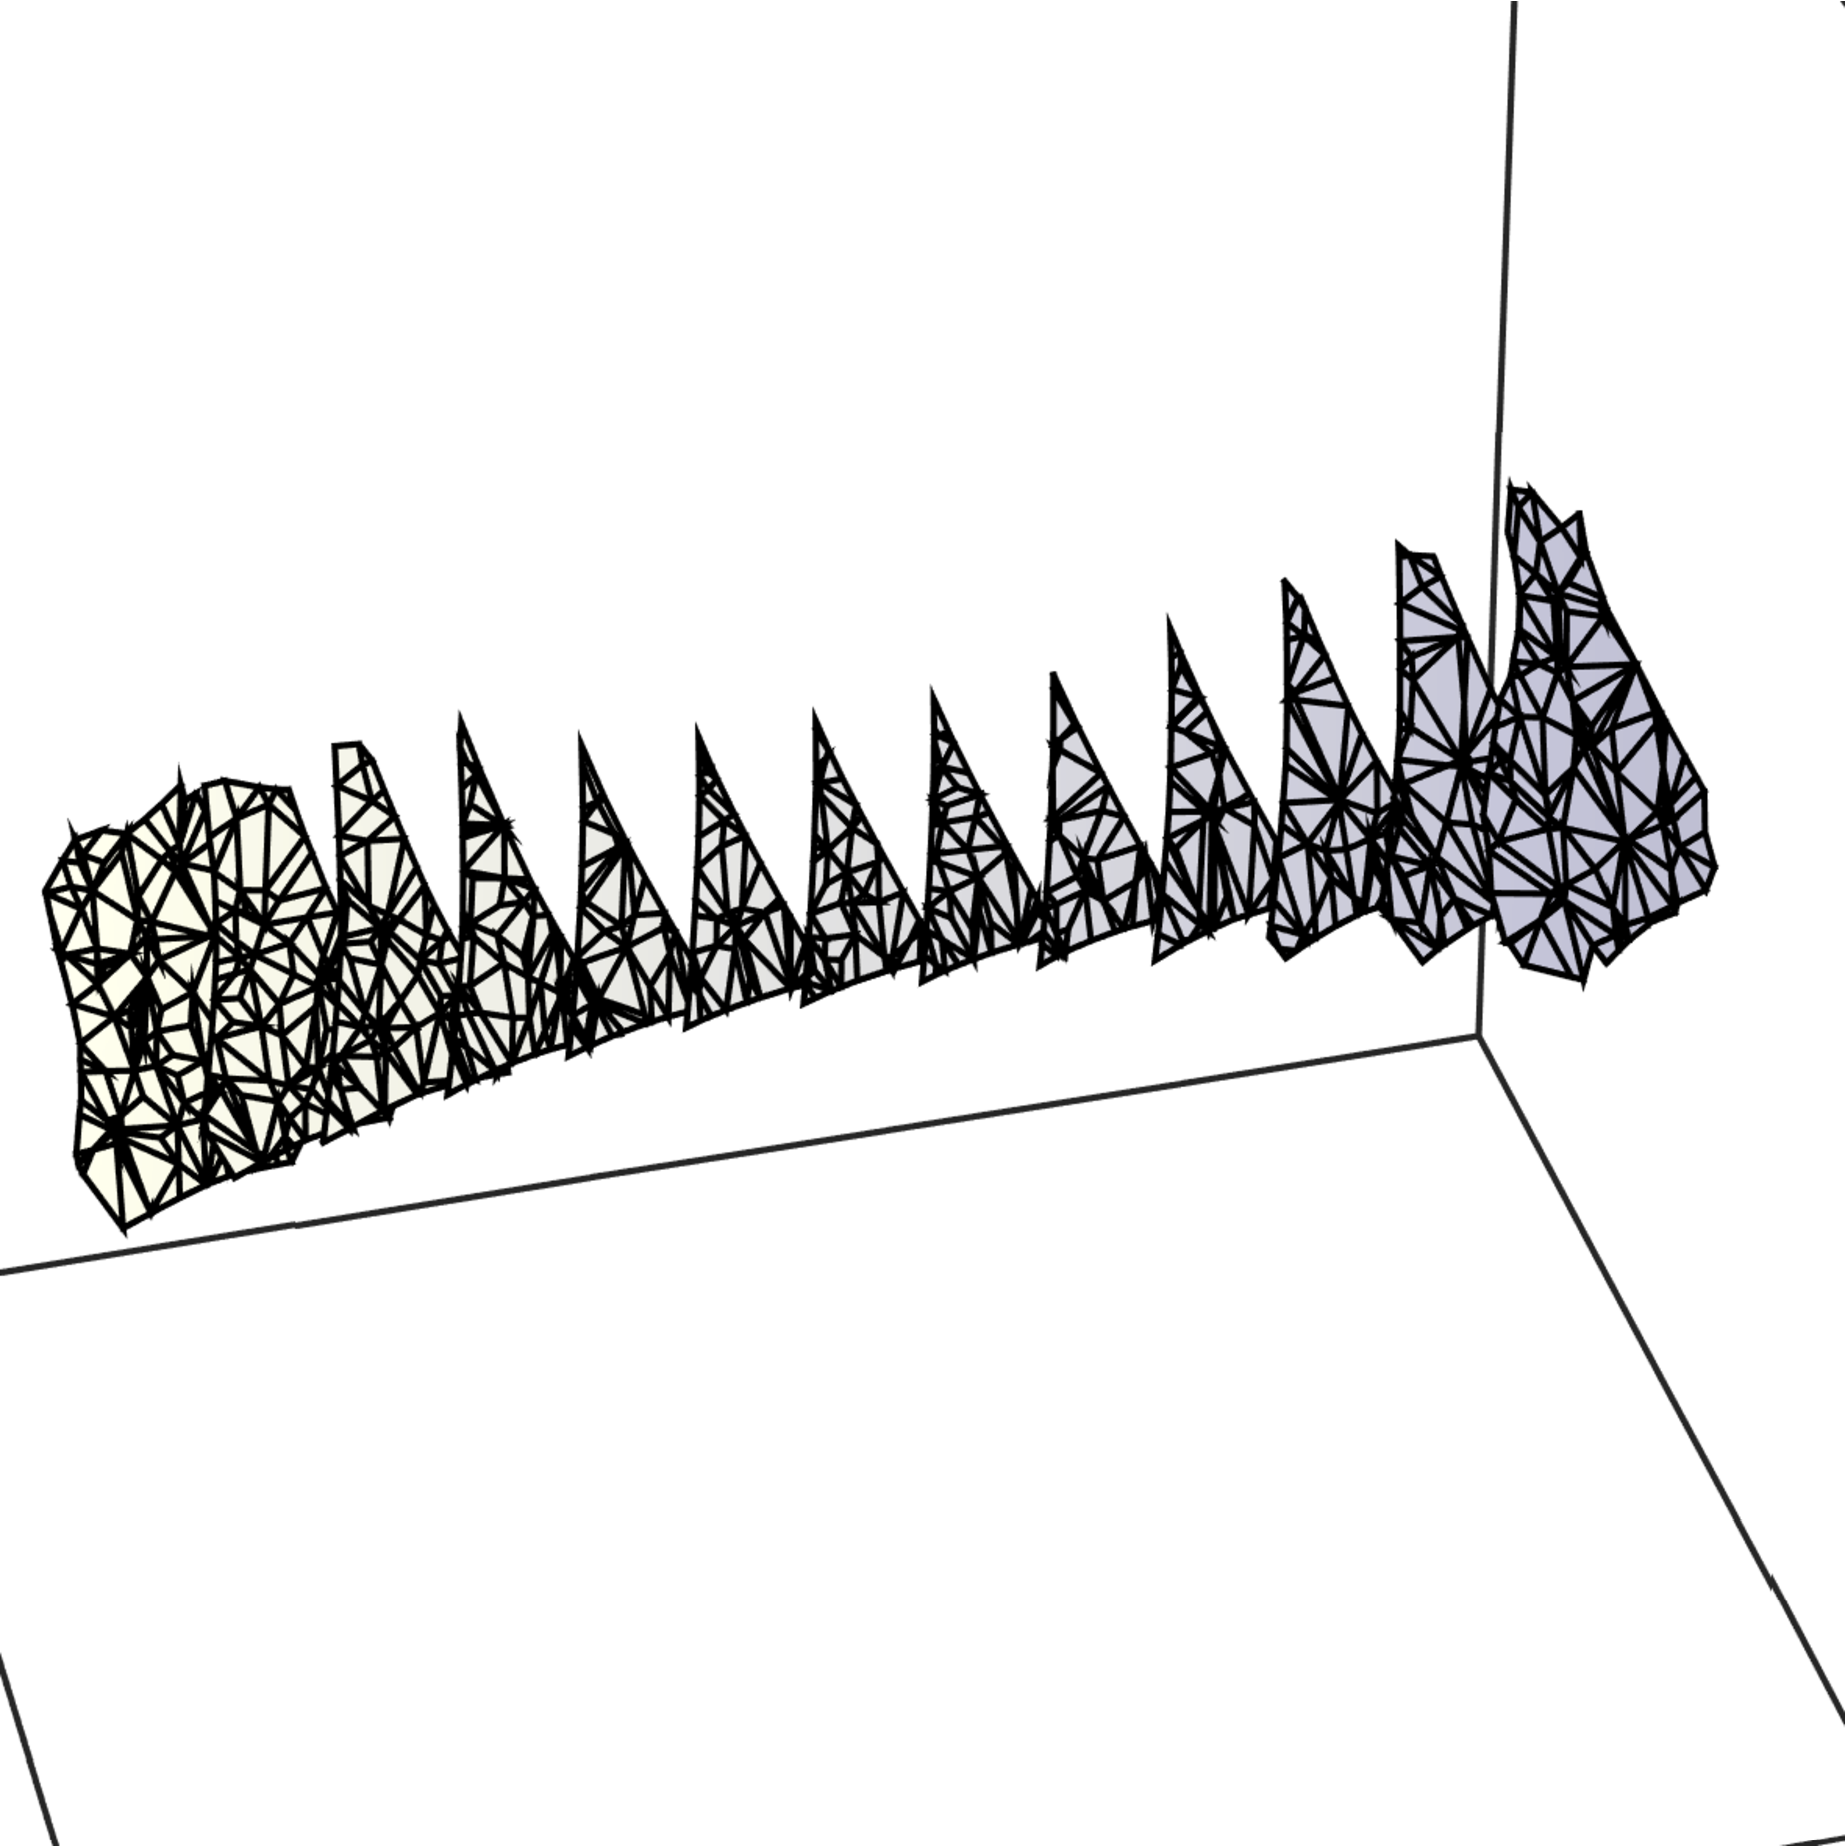
\includegraphics[width=\textwidth]{STRUT_SINGLE_SECTION}
	\end{subfigure}
	\caption{A single sample strut taken from an RVE displaying the behavior of a 20 ppi foam and the cross-section variation comparison at different axial positions.}\label{strut_section}
\end{figure}

\begin{figure}
	\centering
	\begin{subfigure}[b]{0.32\textwidth}
		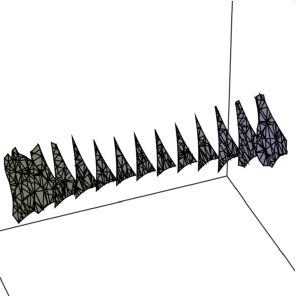
\includegraphics[width=\textwidth]{STRUT_SINGLE_concave_section}
		\caption{{$ k_c = 0.2$}}
	\end{subfigure}
	\begin{subfigure}[b]{0.32\textwidth}
		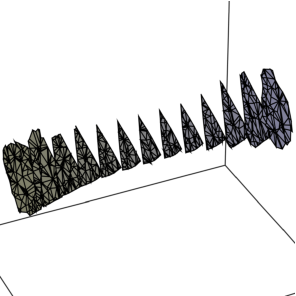
\includegraphics[width=\textwidth]{STRUT_SINGLE_convex_section}
		\caption{{$ k_c = -0.2$}}
	\end{subfigure}
	\begin{subfigure}[b]{0.32\textwidth}
		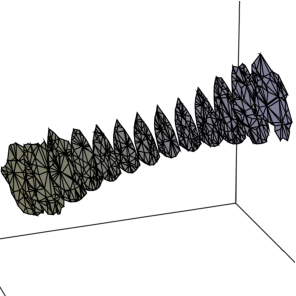
\includegraphics[width=\textwidth]{STRUT_SINGLE_convex2_section}
		\caption{{$ k_c = -0.5$}}
	\end{subfigure}
	\caption{{The cross-section variation comparison by using different concavity paramater, $ k_c $, at mid-span of the struts.}}\label{strut_section_variation}
\end{figure}

\begin{figure}
	\centering
	\begin{subfigure}[b]{0.35\textwidth}
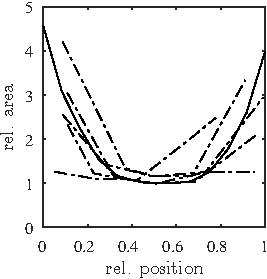
\includegraphics[width=\textwidth]{STRUT_SINGLE_SECTION_PLOT}
	\end{subfigure}
	\caption{A comparison of strut cross-section area with experimental data (in dotted lines, re-sketched from \cite{jungMicrostructuralCharacterisationExperimental2017} for 20 ppi foams), while the bold line depicts the variation for the strut displayed in Figure \ref{strut_section}.}\label{strut_section_plot}
\end{figure}

\begin{table*}[t]
\small{
	\begin{center}
		\caption{Approximate combination of the study of variation of porosity and strut thickness to inclusion radius ratio with ppi based on data on samples of Aluminium foam by ERG and Celltec materials as observed in \cite{perrotPeriodicUnitCell2007} and \cite{jungMicrostructuralCharacterisationExperimental2017}}\label{tab_ppi}
%		\small
		\begin{tabular}{c | c c | c c c c}
			\toprule
			& \multicolumn{2}{c|}{Literature experimental values} & \multicolumn{4}{c}{Values used in DN-RSA}\\[0.5ex]
			\midrule
			
			ppi & Porosity & Average strut thickness &  Values  & Value  &   Average strut thickness to & Obtained \\[0.5ex]
			& in \% \cite{jungMicrostructuralCharacterisationExperimental2017} & to average inclusion  & of [$ c_1 $ $ c_2 $]&of $ k_c $& average inclusion radius & porosity\\[0.5ex]
			& & radius ratio \cite{perrotPeriodicUnitCell2007}& & & ratio for $ t $ in Eq. (\ref{strut7}) &\\[0.5ex]
			\midrule
			5 & - & 0.2310 &- &- &- &-\\[1ex]
			10 & 0.942 & 0.1945&[50 1] &0&0.2050&0.9418 \\[1ex]
			20 & 0.937 & 0.1983& [25 1]&-0.05&0.2&0.9388\\[1ex]
			30 & 0.916 & -&[10 1]&-0.2 &0.198 &0.92\\[1ex]
			40 & - & 0.1878& -& -& -&-\\[1ex]
			\bottomrule
		\end{tabular}
	\end{center}}
\end{table*}



%It is common to obtain foams that exhibit anisotropy with a preferential direction in the rise direction of the initial PU foam \cite{jungMicrostructuralCharacterisationExperimental2017}. This can be modeled by simply introducing an anisotropy in the distance functions. It is also possible to introduce anisotropy in the initial sphere packings, as demonstrated in \cite{sononAdvancedApproachGeneration2015}, but this would not achieve optimal close packing due to the principle underlying DN-RSA.

\subsubsection{Generation of targeted morphology}
From values reported in Table \ref{tab_ppi}, it can be seen that the standard values for porosity with varying ppi are quite dispersed statistically. However, a linear correlation can be used for the sake of simplicity. Since the samples in these studies are mono-dispersed open-cell Aluminium foams, a closed packing  of nearly mono-dispersed spheres can be generated using DN-RSA. Once the packing of spheres is generated, based on individual tessellation volumes, the mean characteristic length of the inclusions can be obtained. This value can be combined with the thickness to radius ratio obtained in Table \ref{tab_ppi} and the respective values of coefficient $ c_1 $, $ c_2 $ and $ k_c $ depending on the ppi to generate an open foam RVE. Simple interpolation can be used for values that lie in between. The final column of Table \ref{tab_ppi} shows that the porosity values obtained match to a good extent, while maintaining the morphological similarity of the RVE foam with real foam samples.
%The quantification of some of the important parameters in this section shows high similarity with the existing works done in the study of Laguerre tessellation and fitting these models to foam samples. In the case of largely mono-disperse foams, the RVEs developed following DN-RSA show similarities to the models developed by already existing tools along with operators and tools to implement strut morphology variations and development of coated layers. By comparing a single RVE with a sample foam, the starting parameters can be set and multiple RVEs can be generated to enable the development of a statistical study of the mechanical properties of the RVEs, in a comparatively shorter amount of time without using too much of computational power.

{Figure \ref{anisotropy} shows the implementation of the anisotropy parameter (in percentage) along X axis on the packing to extract anisotropic morphologies from a single DN-RSA packing as described in Section \ref{of-feature-anisotropy}. This parameter is particularly helpful in implicitly implementing the anisotropy that is observed in actual foams due to the solidification of cast metal in the rise direction.}

\begin{figure}
	\centering
	\begin{subfigure}[b]{0.32\textwidth}
		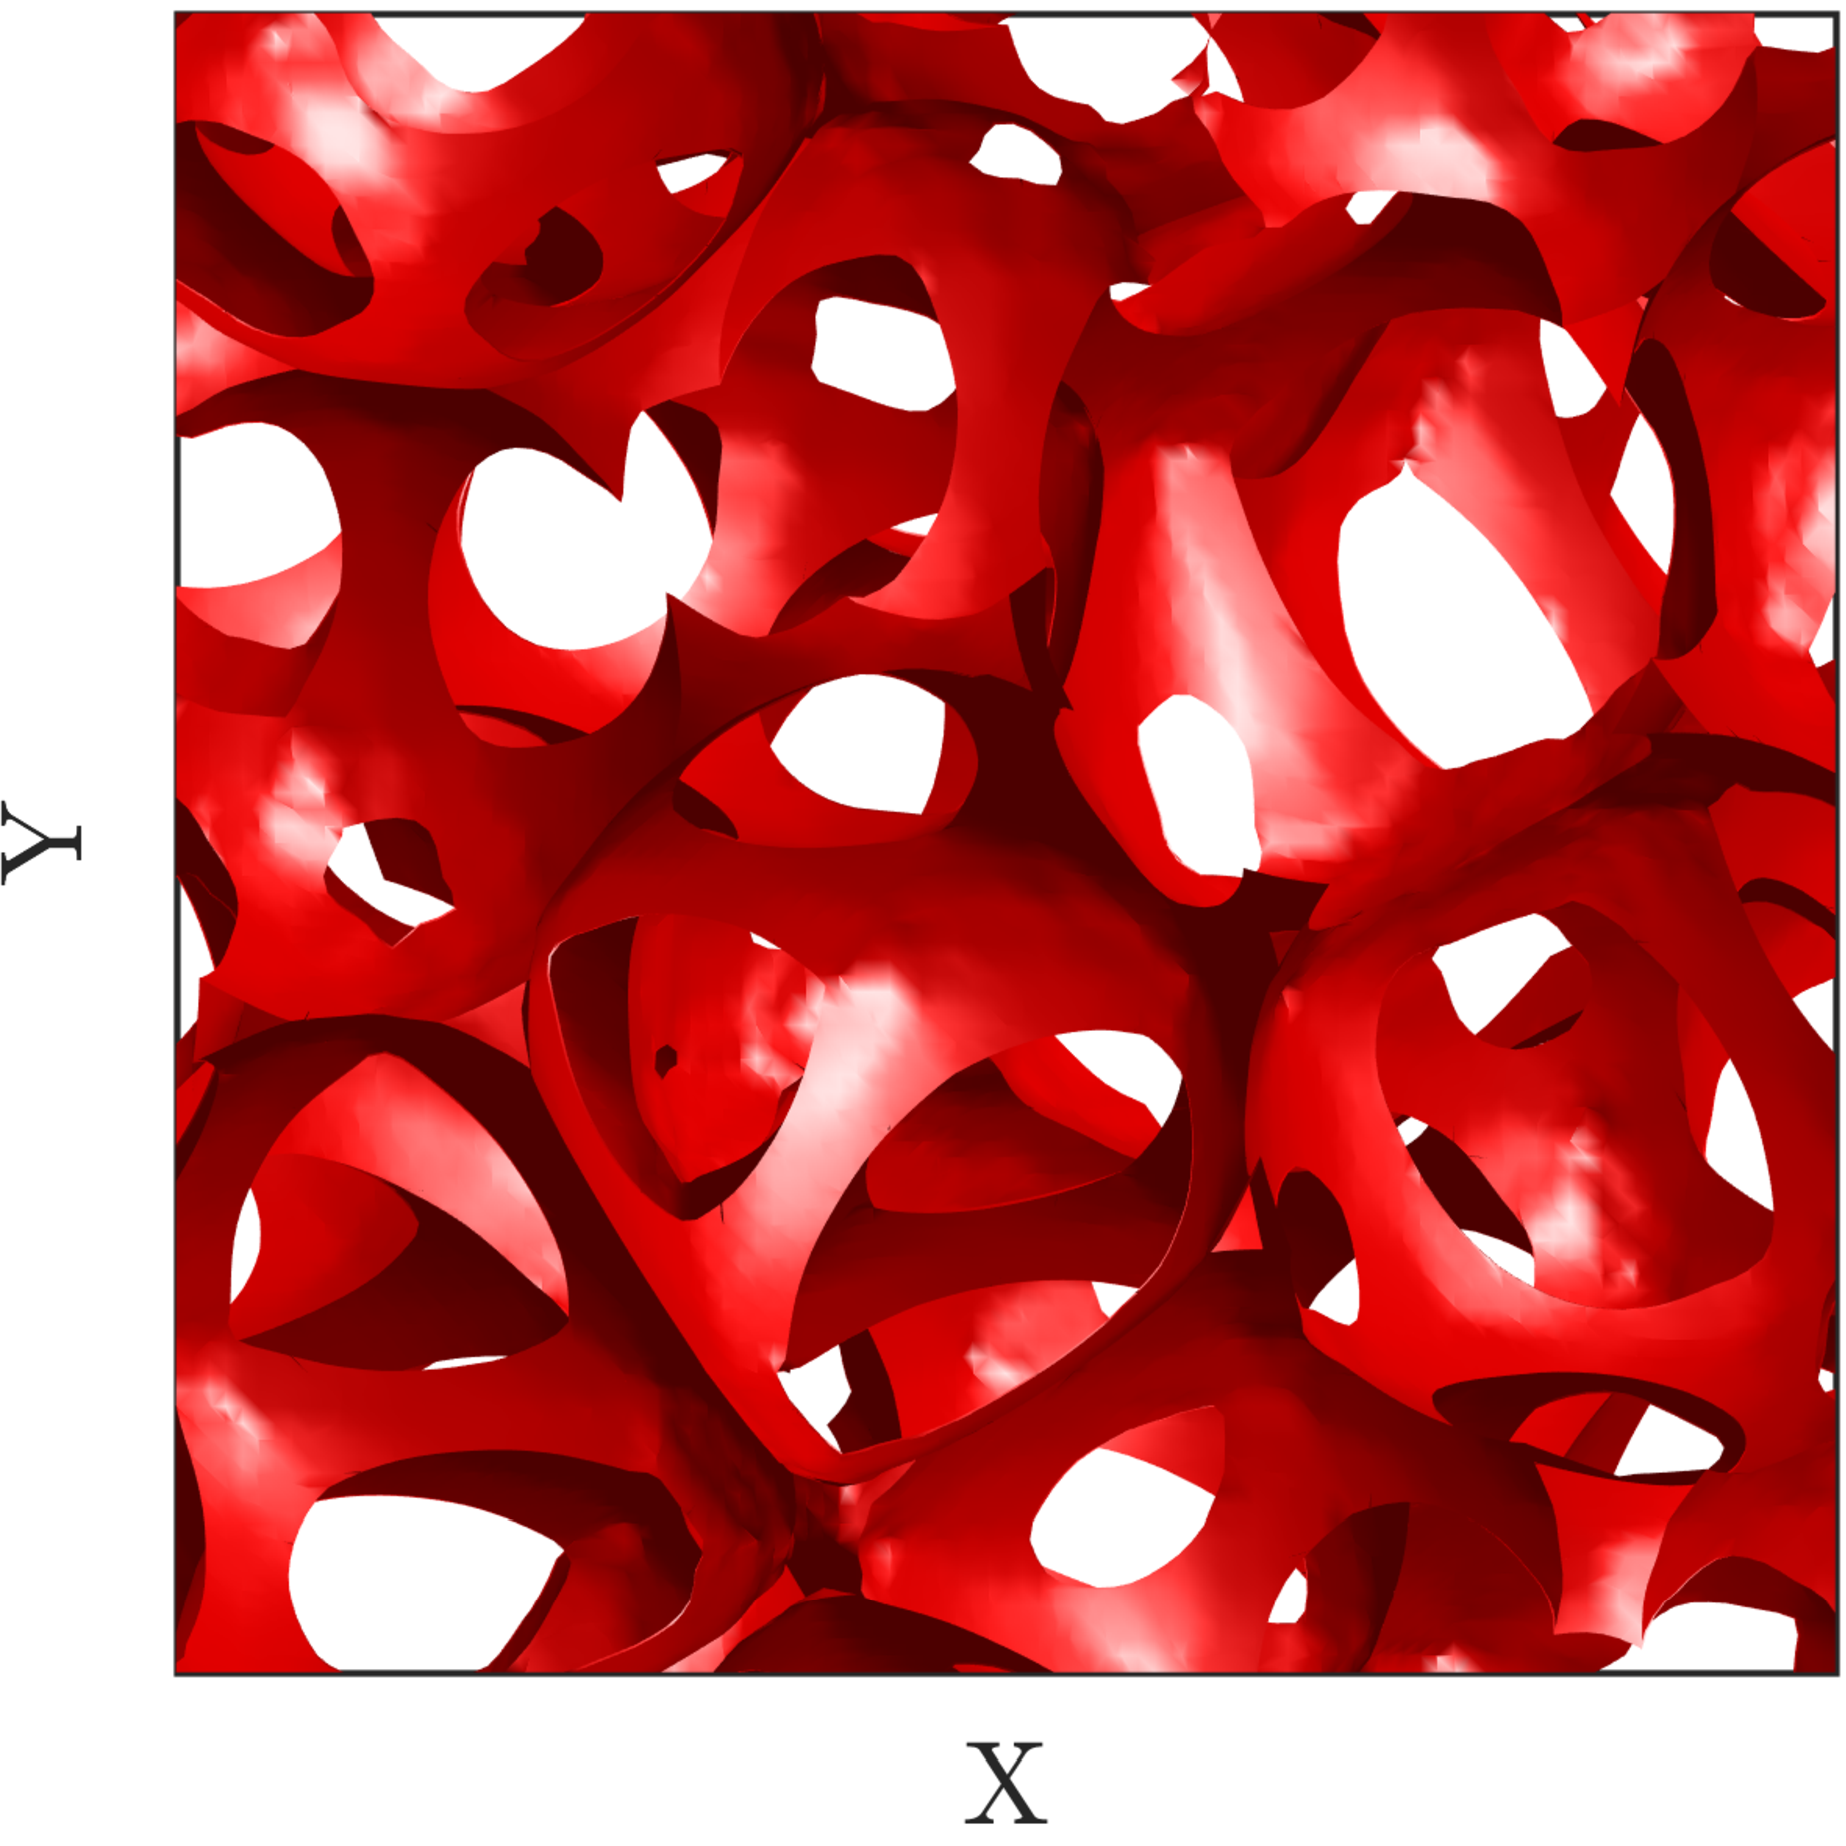
\includegraphics[width=\textwidth]{anisotropy_1}
		\caption{{No anisotropy}}
	\end{subfigure}
	\begin{subfigure}[b]{0.32\textwidth}
		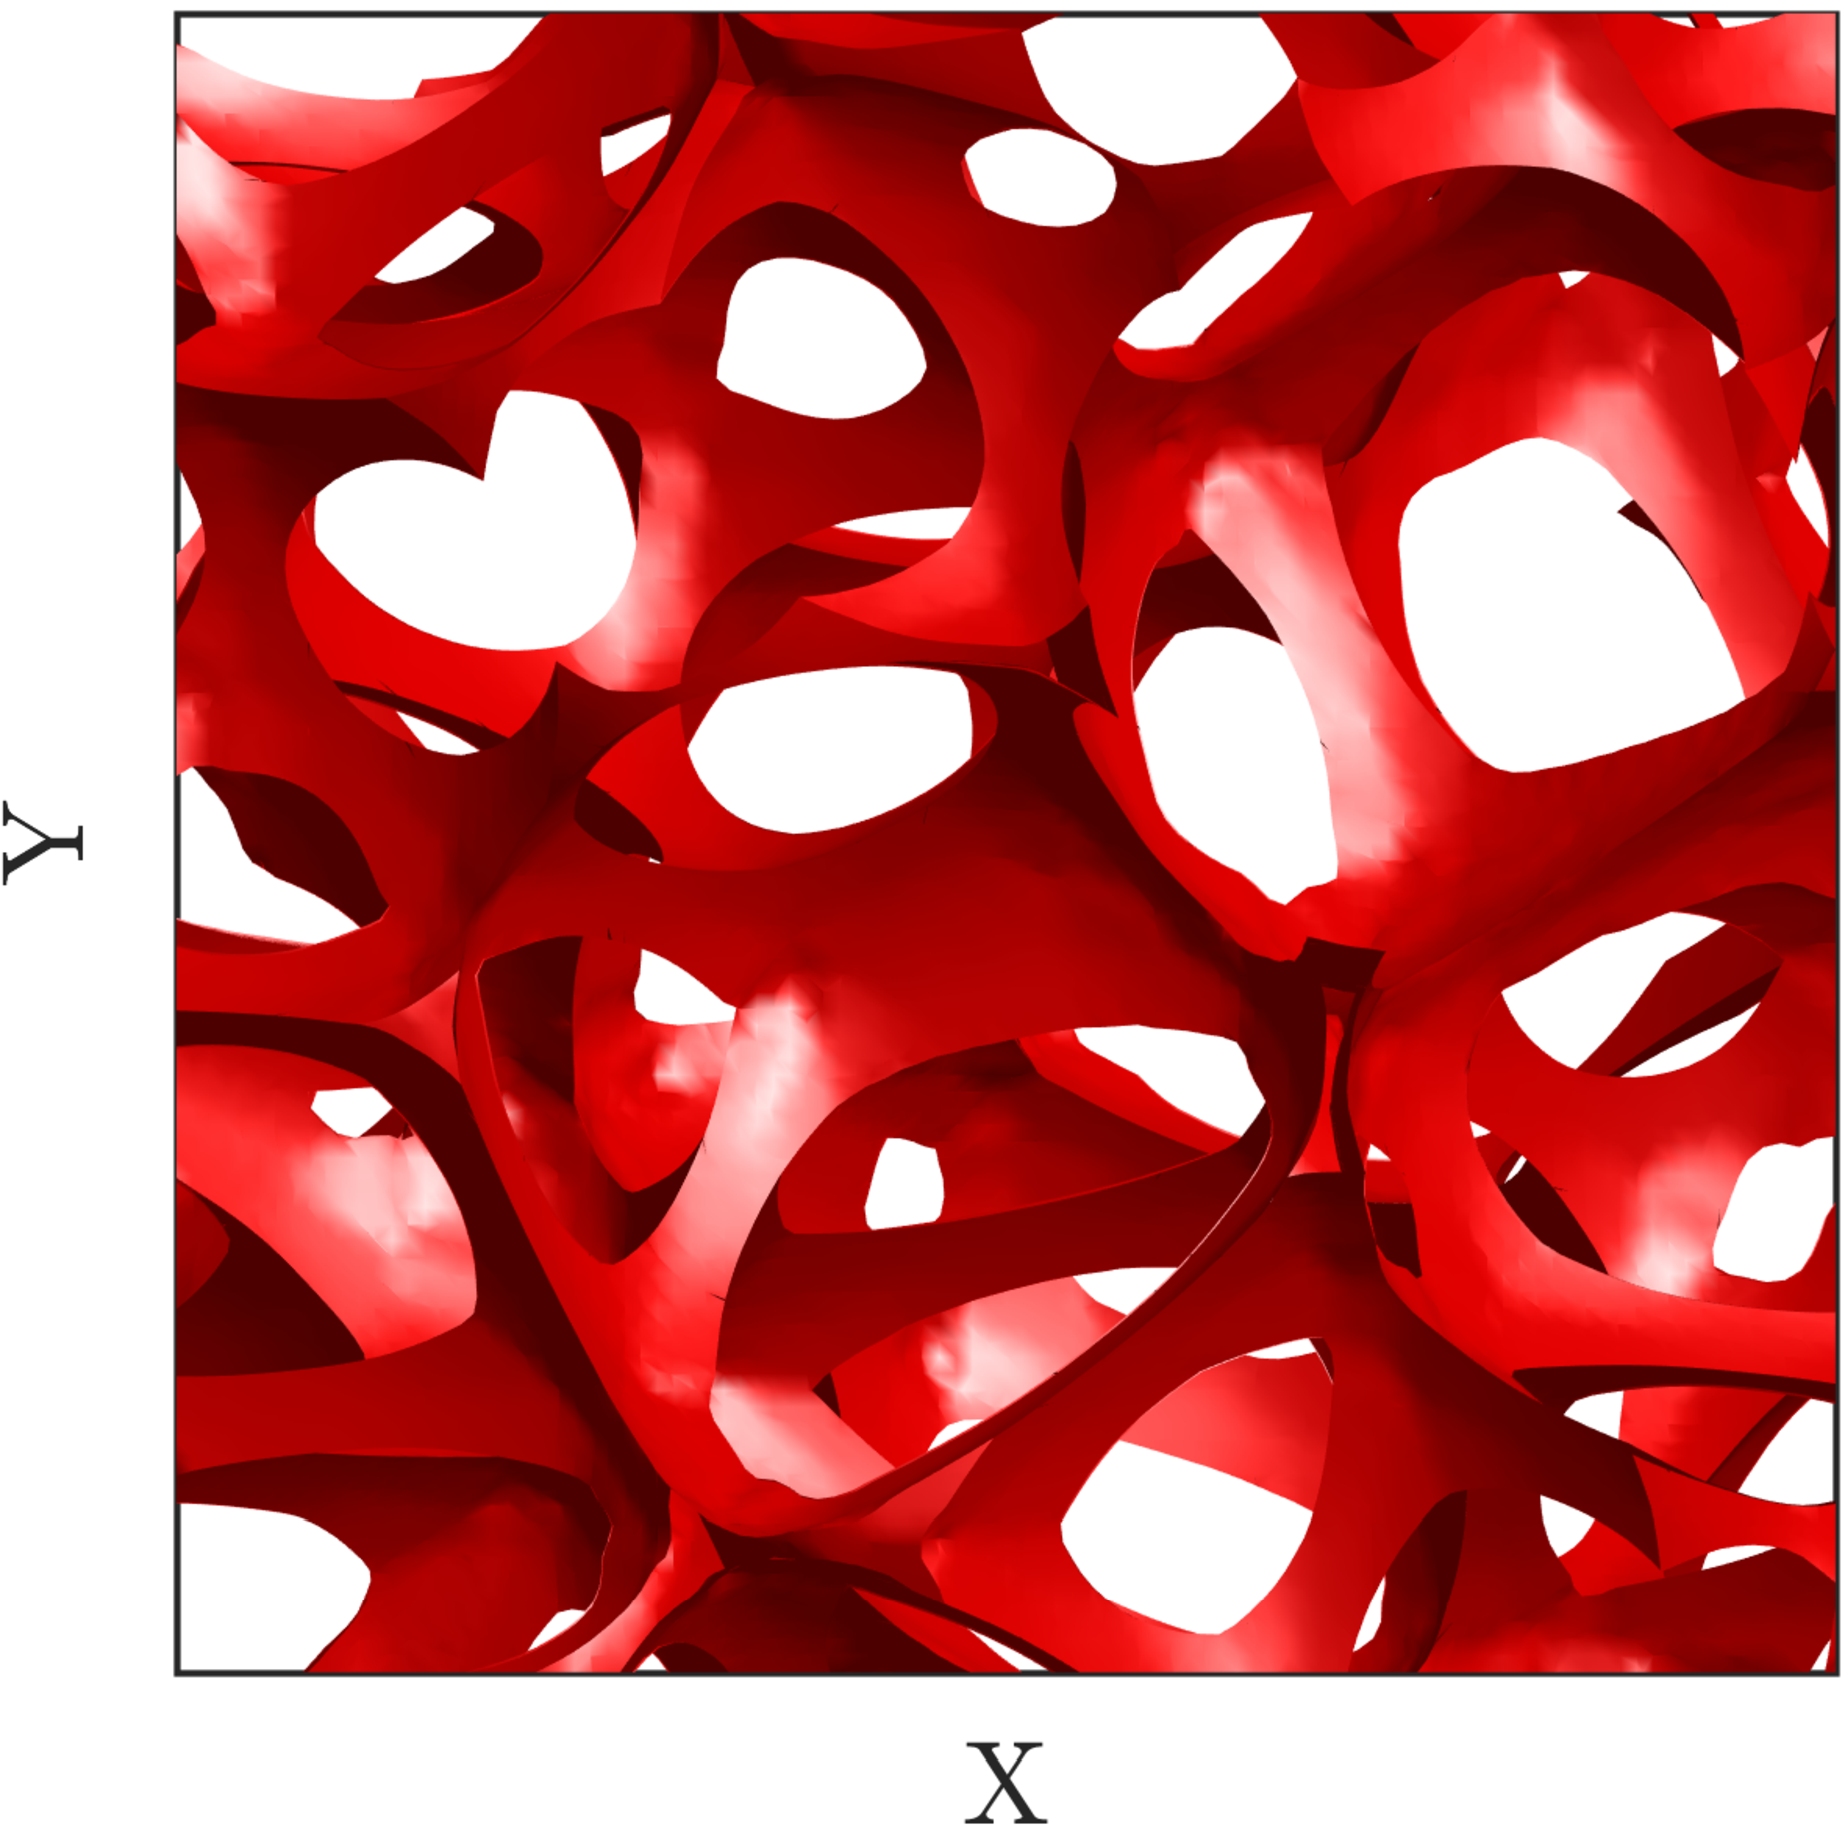
\includegraphics[width=\textwidth]{anisotropy_2}
		\caption{{25\% anisotropy}}
	\end{subfigure}
	\begin{subfigure}[b]{0.32\textwidth}
		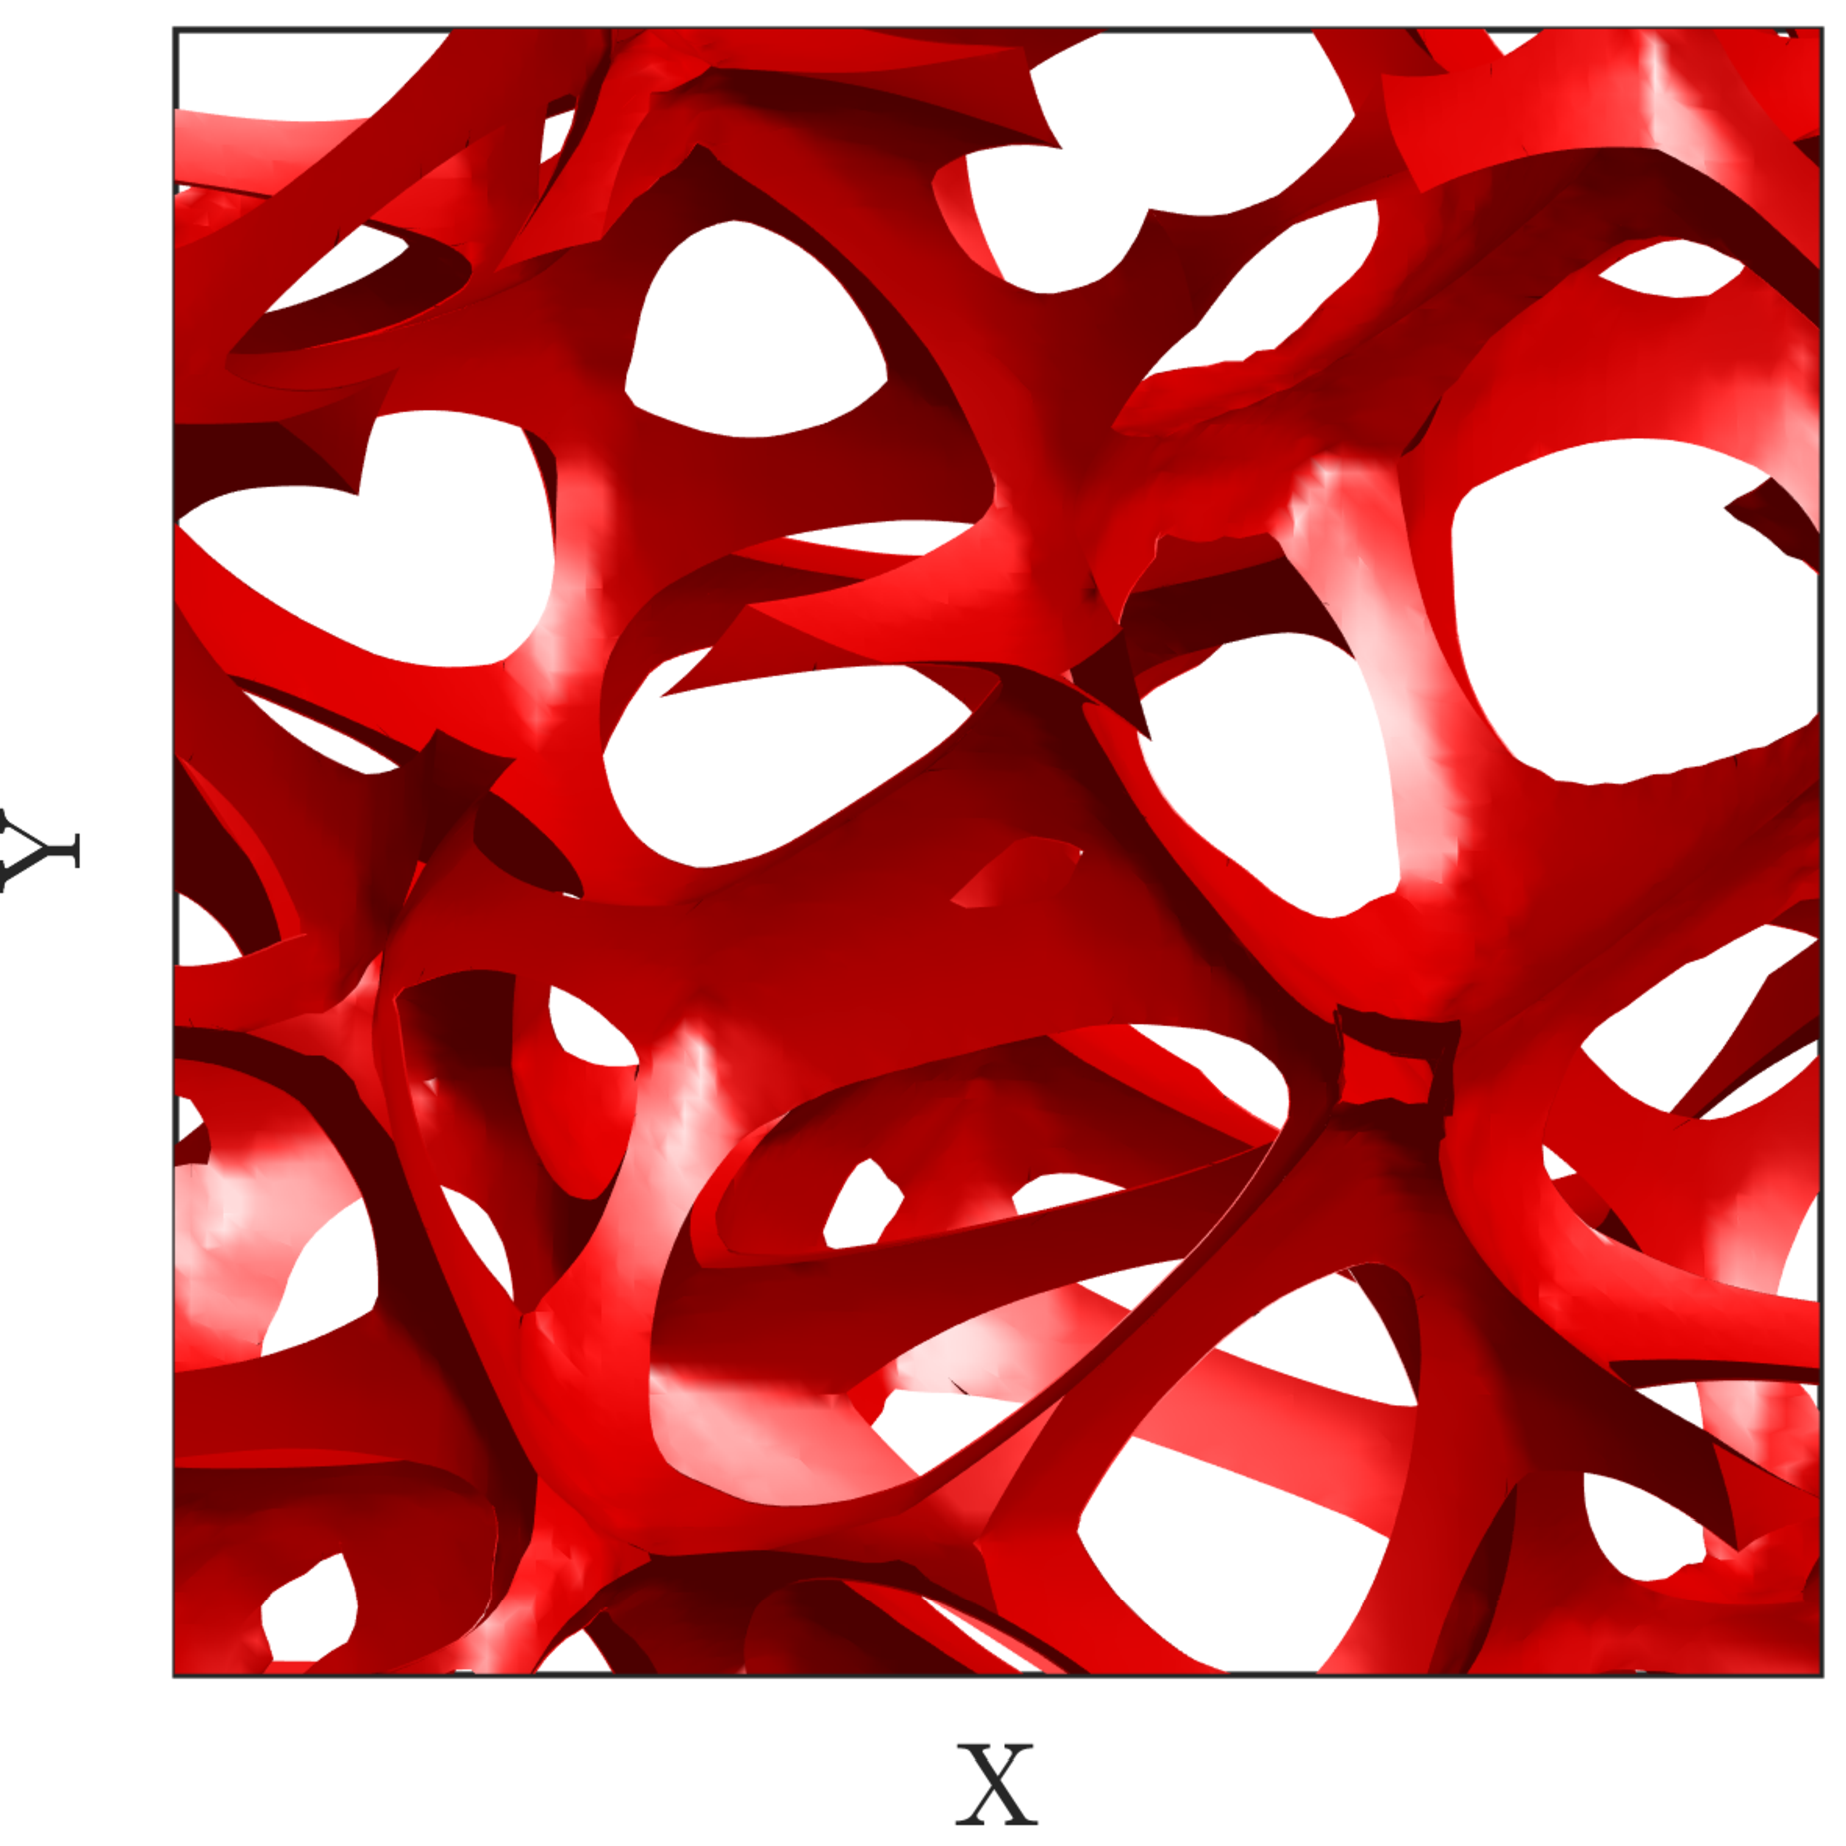
\includegraphics[width=\textwidth]{anisotropy_3}
		\caption{{50\% anisotropy}}
	\end{subfigure}
	\caption{{Implementation of anisotropy variation on a foam generated from a single DN-RSA packing along X axis.}}\label{anisotropy}
\end{figure}

\red{In a discrete set-up, one needs to mention the utility of using a set discretization size. Lower discretization size results in achieving higher accuracy in the geometries generated, at the same time increasing the computational cost due to the higher number of grid points and the related complexities this results in. The systems consume higher memory to store the information at all these grid points and the overall morphology generation process slows down. In our experience, it is sufficient to proceed with a grid size of $ 100\times100\times100 $ and still achieve qualitative results.}

\red{With the availability of more data coming from various manufacturers of open foams, a better relationship can be established between the geometry generation parameters, like $ c_1$, $c_2$, $ k_c $, $ t $ and ppi values. This can not only help in obtaining better geometries, but also in establishing a clear pattern of the materiel behavior of these morphologies. }

\section{Discussions on morphology reconstructed from CT-scans}\label{res-ct}
\sectionmark{CT-scans reconstructions}
The RSA algorithm to generate random packing of ellipsoids and arbitrary shaped inclusion is a computationally expensive process due to a lack of a closed form distance to these inclusions. Also, unlike the spherical packing, ellipsoids or arbitrary shaped inclusion packing does not result in a closed packing as the methodology uses circumscribed spheres in the distance field assisted packing where the optimal orientation of the inclusion is not considered in the packing. In light of this knowledge, it would be interesting to compare the ellipsoid and polyhedral based morphologies developed from an actual foam sample as the basis using DN-CT-SCAN with the experimental observations, considering that the inclusion generation is a zero cost computation process as far as DN-CT-SCAN is concerned. An RSA based packing of spherical inclusions would be an ideal candidate to test the statistical validity of the generated morphologies considering its easy, low cost generation using DN-RSA, whereas the information rich ellipsoid and polyhedral based packing is ideal to test DN-CT-SCAN as a reconstruction tool. 

Following the reconstruction process explained in Section \ref{of-CT}, it is possible to obtain the geometry of an open foam sample from CT-scan images. In this aspect, a set of CT scan images of a 20 ppi aluminium open foam sample was provided by the Chair of Technical Mechanics in University of Saarland. Based on the methodology presented in Section \ref{res-random} to quantify the morphology, it is possible to analyze in a similar manner the various indicators that can be extracted from the reconstructed geometry. By using the algorithm explained in \cite{leblancAnalysisOpenFoamUnderPreparation}, it is possible to obtain initially a set of ellipsoids that can be embedded inside the image of the specimen. Once the ellipsoids are available, a set of reference polyhedrals can be recovered. Morphological indicators of reconstructions based on the ellipsoids as well as polyhedrals will be compared here.

\begin{figure}
	\centering
	\begin{subfigure}[b]{0.45\textwidth}
		\includegraphics[width=\textwidth]{polyhedra_ct-scan}
	\end{subfigure}
	\begin{subfigure}[b]{0.45\textwidth}
		\includegraphics[width=\textwidth]{polyhedra_ct-scan_view3}
	\end{subfigure}
	\caption{CT-scan (red) data embedded in the reconstructed geometry (blue) extracted using polyhedral basis compared visually.}\label{res-ct-visual}
\end{figure}

Figure \ref{res-ct-visual} illustrates a comparison of the visual features between the CT scan image voxels (in red) and the geometry extracted from the underlying polyhedrals (in blue). Visually, the geometry is quite close to the physical samples. The sample under consideration is made of around 600 voxels in each direction with each voxel of size $ 24\times24\times24\,\mu\text{m}^3 $ . This gives an effective cube of 14.4mm in each direction. The geometry of the struts, including the strut curvature and cross section variation, has been achieved using the values established in Table \ref{tab_ppi} for a foam of 20 ppi. By counting the active voxels, the porosity of the foam was found to be 93\%. The porosity of the geometry extracted from the underlying polyhedrals was found to be 92.7\% using the ``implicit'' approach and 93.2\% using the ``classical'' approach.

This sample then results in around 15 pores that are completely surrounded by other pores in the sample. Figure \ref{res-ct-face}(a) illustrates the number of faces per pore using different approaches. It can be seen that the number of pores necessary to obtain an effective comparison is not available with the given sample. However on taking the number of edges per face, as illustrated in Figure \ref{res-ct-face}(b), the data obtained by QHull software and the classical approach for the polyhedral based reconstruction match really well. This confirms with the visual findings between the CT scan images and the polyhedral based extraction. 

Figure \ref{res-ct-edge} illustrates the edge length distribution of the reconstructed geometry. It can be seen that the QHull method overestimates the number of short length edges while with the classical approach, this is greatly reduced, due to reasons as explained in Section \ref{res-random}. The geometry obtained using the polyhedral basis has been chosen here considering that it represents the physical morphology closer than the one obtained using the ellipsoids.

\begin{figure}
	\centering
	\begin{subfigure}[b]{0.49\textwidth}
		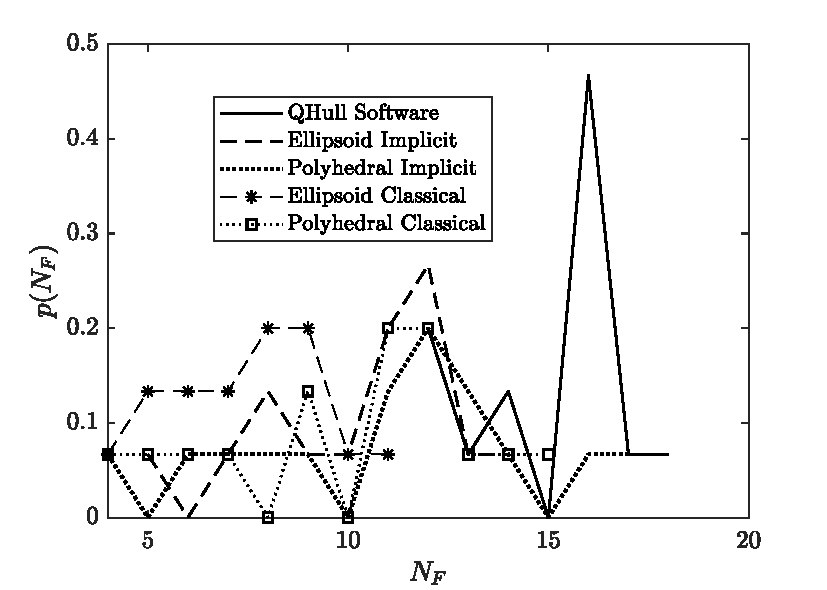
\includegraphics[width=\textwidth]{ct_scan_face_3}
		\caption{}
	\end{subfigure}
	\begin{subfigure}[b]{0.49\textwidth}
		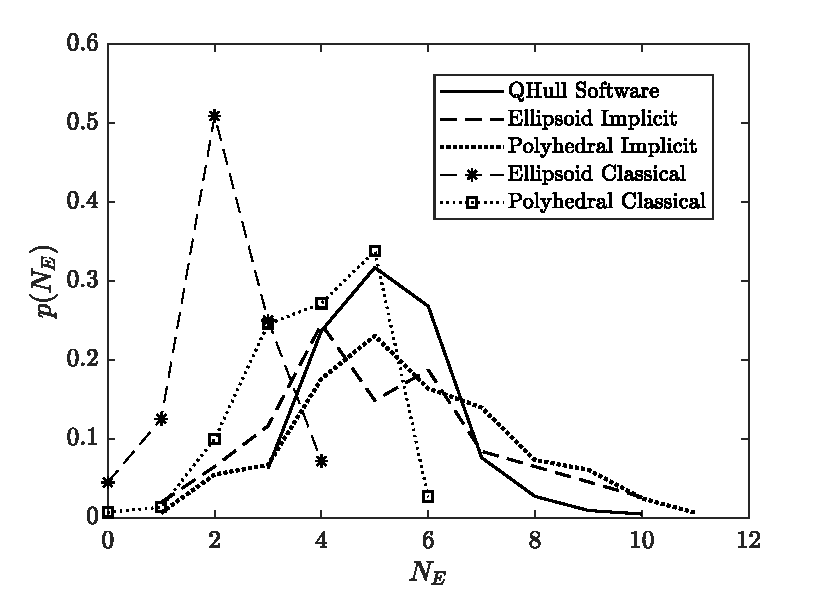
\includegraphics[width=\textwidth]{ct_scan_edge_3}
		\caption{}
	\end{subfigure}
	\caption{(a) Comparison of the occurrence of the number of faces per pore using various approaches, and (b) Comparison of the occurrence of the edges per face using various approaches, for the reconstructed morphology using DN-CT-SCAN. }\label{res-ct-face}
\end{figure}

\begin{figure}
	\centering
	\begin{subfigure}[b]{0.49\textwidth}
		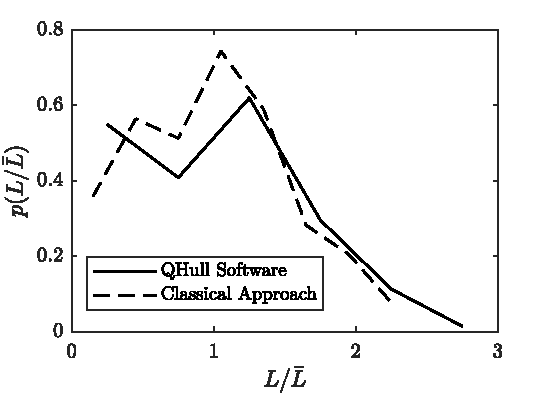
\includegraphics[width=\textwidth]{ct_scan_edge_len}
	\end{subfigure}
	\caption{Normalized edge length distribution of the reconstructed morphology using DN-CT-SCAN. Comparison is drawn between the QHull software results obtained using the seeds of the ellipsoids/polyhedrals and the classical approach applied on the geometry extracted using the polyhedral basis.}\label{res-ct-edge}
\end{figure}

It is true that the sample size available is not sufficient to draw a  definitive conclusion, but with the help of available visual tools and comparison of key-identifiers, one can reconstruct the geometry of foam morphology to a satisfactory extent using the CT scan as a basis in the DN-CT-SCAN algorithm. Considering that the resultant finite element models can be extracted with ease using this methodology, the combination of polyhedrals packing with DN-CT-SCAN can be a quick alternative to other complex and computationally expensive methodologies to obtain voxel based finite element models when the latter also suffer from the presence of spurious stress concentration due to the 
%TODO ensure this doesn't end in next page
jagged boundaries of the voxels. 
\enlargethispage{\baselineskip}

\section{Finite element modeling of the com\-pres\-sive response of foams}\label{res-fem}
\sectionmark{FEM of compressive response of foams}
In this section, a finite element simulation is conducted to demonstrate the ability of the RVE generation procedure to reproduce the structural properties of open foam. First, a sample micro-cell is generated based on morphological parameters of an open foam sample available from literature \cite{jungMicrostructuralCharacterisationExperimental2017}. Material parameters identified in \cite{heinzeExperimentalNumericalInvestigation2018} are used for the struts' constitutive model. A single pore will be identified initially and a compression test will be simulated. The results will be compared with that reported in \cite{heinzeExperimentalNumericalInvestigation2018}. Then an entire generated RVE obtained using the DN-RSA algorithm, is computed under a uniaxial compression, using the finite element procedures proposed in \cite{nguyenComputationalHomogenizationCellular2014,nguyenUnifiedTreatmentMicroscopic2017} and a comparison is built between the model predictions and the experimental data provided in \cite{jungMicrostructuralCharacterisationExperimental2017}. Finally, the geometries reconstructed from the CT-scans based polyhedrals and ellipsoids using DN-CT-SCAN are tested against experimental tests conducted on the original foam material as observed in \cite{jungMicrostructuralCharacterisationExperimental2017}.

\subsection{RVE obtained using DN-RSA}\label{res-fem-rsa}
\subsubsection*{Generation of RVE}
An RVE of open foam is prepared which mimics the morphology of Aluminum foam investigated under uniaxial compression in \cite{jungMicrostructuralCharacterisationExperimental2017}. The generation uses the DN-RSA procedure with non-periodic conditions and mono-dispersed volumes of an initial sphere packing with around 125 spheres in the RVE. After minus-sampling, around 25 inclusions remain in the RVE. The radii of the spheres in the packing are randomly chosen from a logarithmic distribution with a CV of 0.07 and a mean radius of 0.125mm. The strut morphology is varied to match the ppi of the foam with which it is compared. With the help of Figure \ref{density_t} and Table \ref{tab_ppi}, appropriate values can be selected to mimic a foam with ppi between 20 and 30 with $ c_1=20 $, $ c_2=1 $ and $ k_c=-0.1 $. Additionally, an anisotropy in the pore geometry is also introduced during the minus-sampling along the direction in which the uniaxial test is  conducted to mimic the anisotropy present along the rise direction during the manufacturing phase. In this case, based on the experimental observations in \cite{jungMicrostructuralCharacterisationExperimental2017}, we propose an anisotropy coefficient of 1.4 along the rise direction. 

For illustration, the struts obey a linear hardening hy\-per\-elas\-tic-based \textit{J}$_2 $-elasto-plastic material law formulated in large strains (Appendix A of \cite{nguyenComputationalHomogenizationCellular2014}), with the isotropic hardening law
\[ \sigma_y^0(\bar{\varepsilon}^{pl}) =\sigma_0+H_{iso}\bar{\varepsilon}^{pl}.
\]
Standard bulk material properties of AlSi7Mg0.3 alloy are in general much higher than those identified in experimental tests on foamed materials \cite{heinzeExperimentalNumericalInvestigation2018} using experimental force-displacement diagrams. This is due to the differences in the foams manufacturing process that cause changes in grains structure and texture. In \cite{heinzeExperimentalNumericalInvestigation2018}, the authors used an inverse identification of the struts material properties from the compression test based on a single pore, which served as a geometric model of an FE simulation. We use the average identified values of $ E=3968.12 $ MPa, $ \sigma^0=46.35 $ MPa, and $ H_{iso}=214.61 $ MPa.


\subsubsection*{Single pore simulations}
\begin{figure}
	\centering
	\begin{subfigure}[b]{0.33\textwidth}
		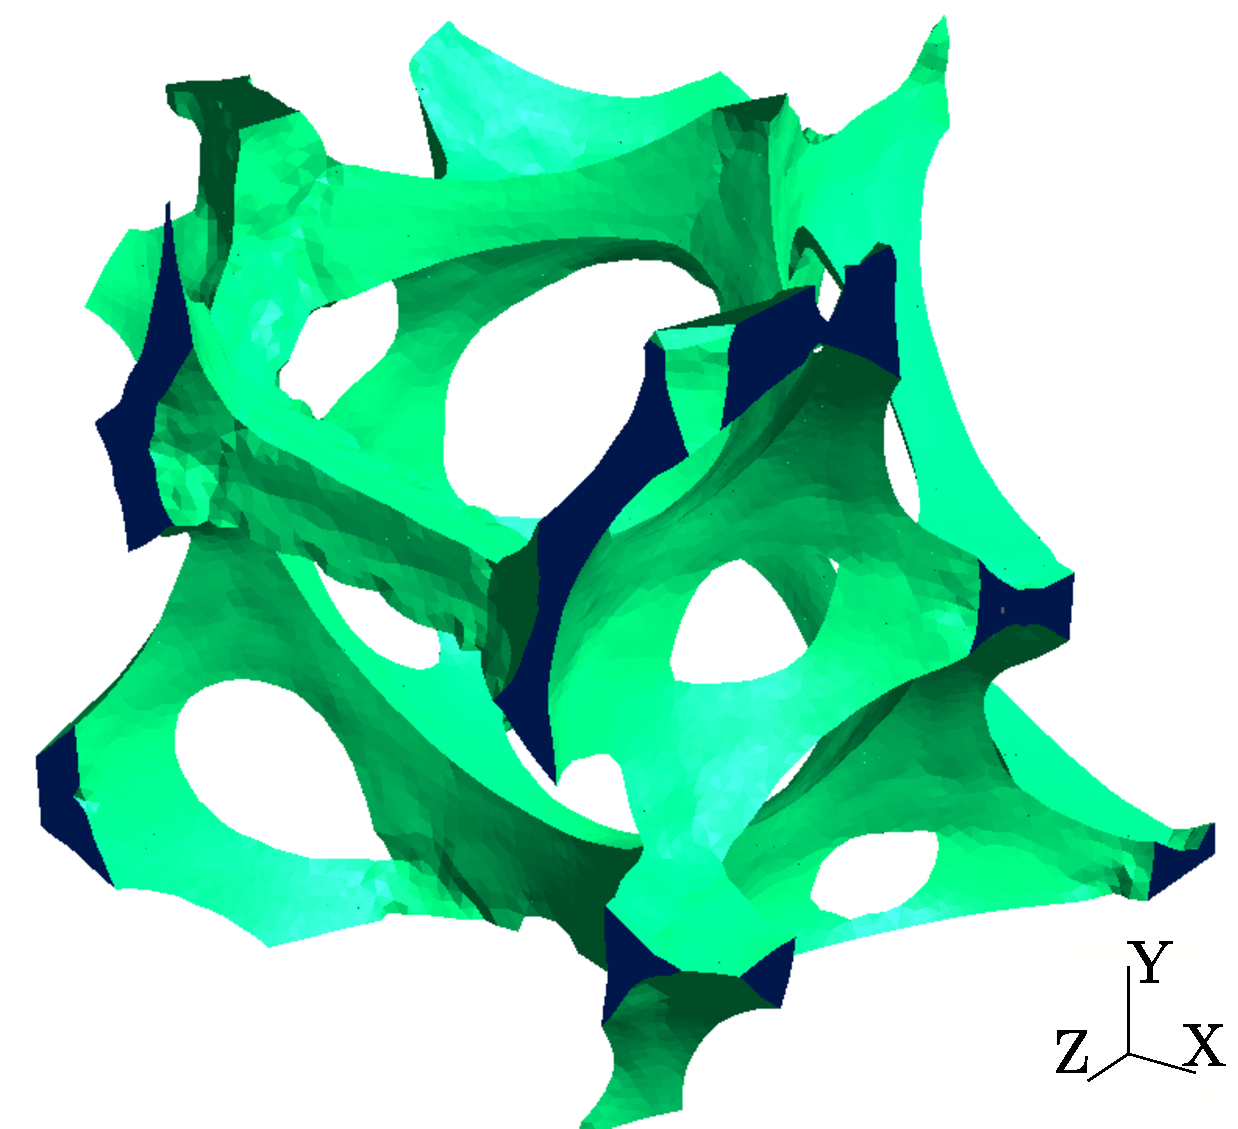
\includegraphics[width=\textwidth]{SIMPLE_MESH}
		\caption{}
	\end{subfigure}
	\begin{subfigure}[b]{0.33\textwidth}
		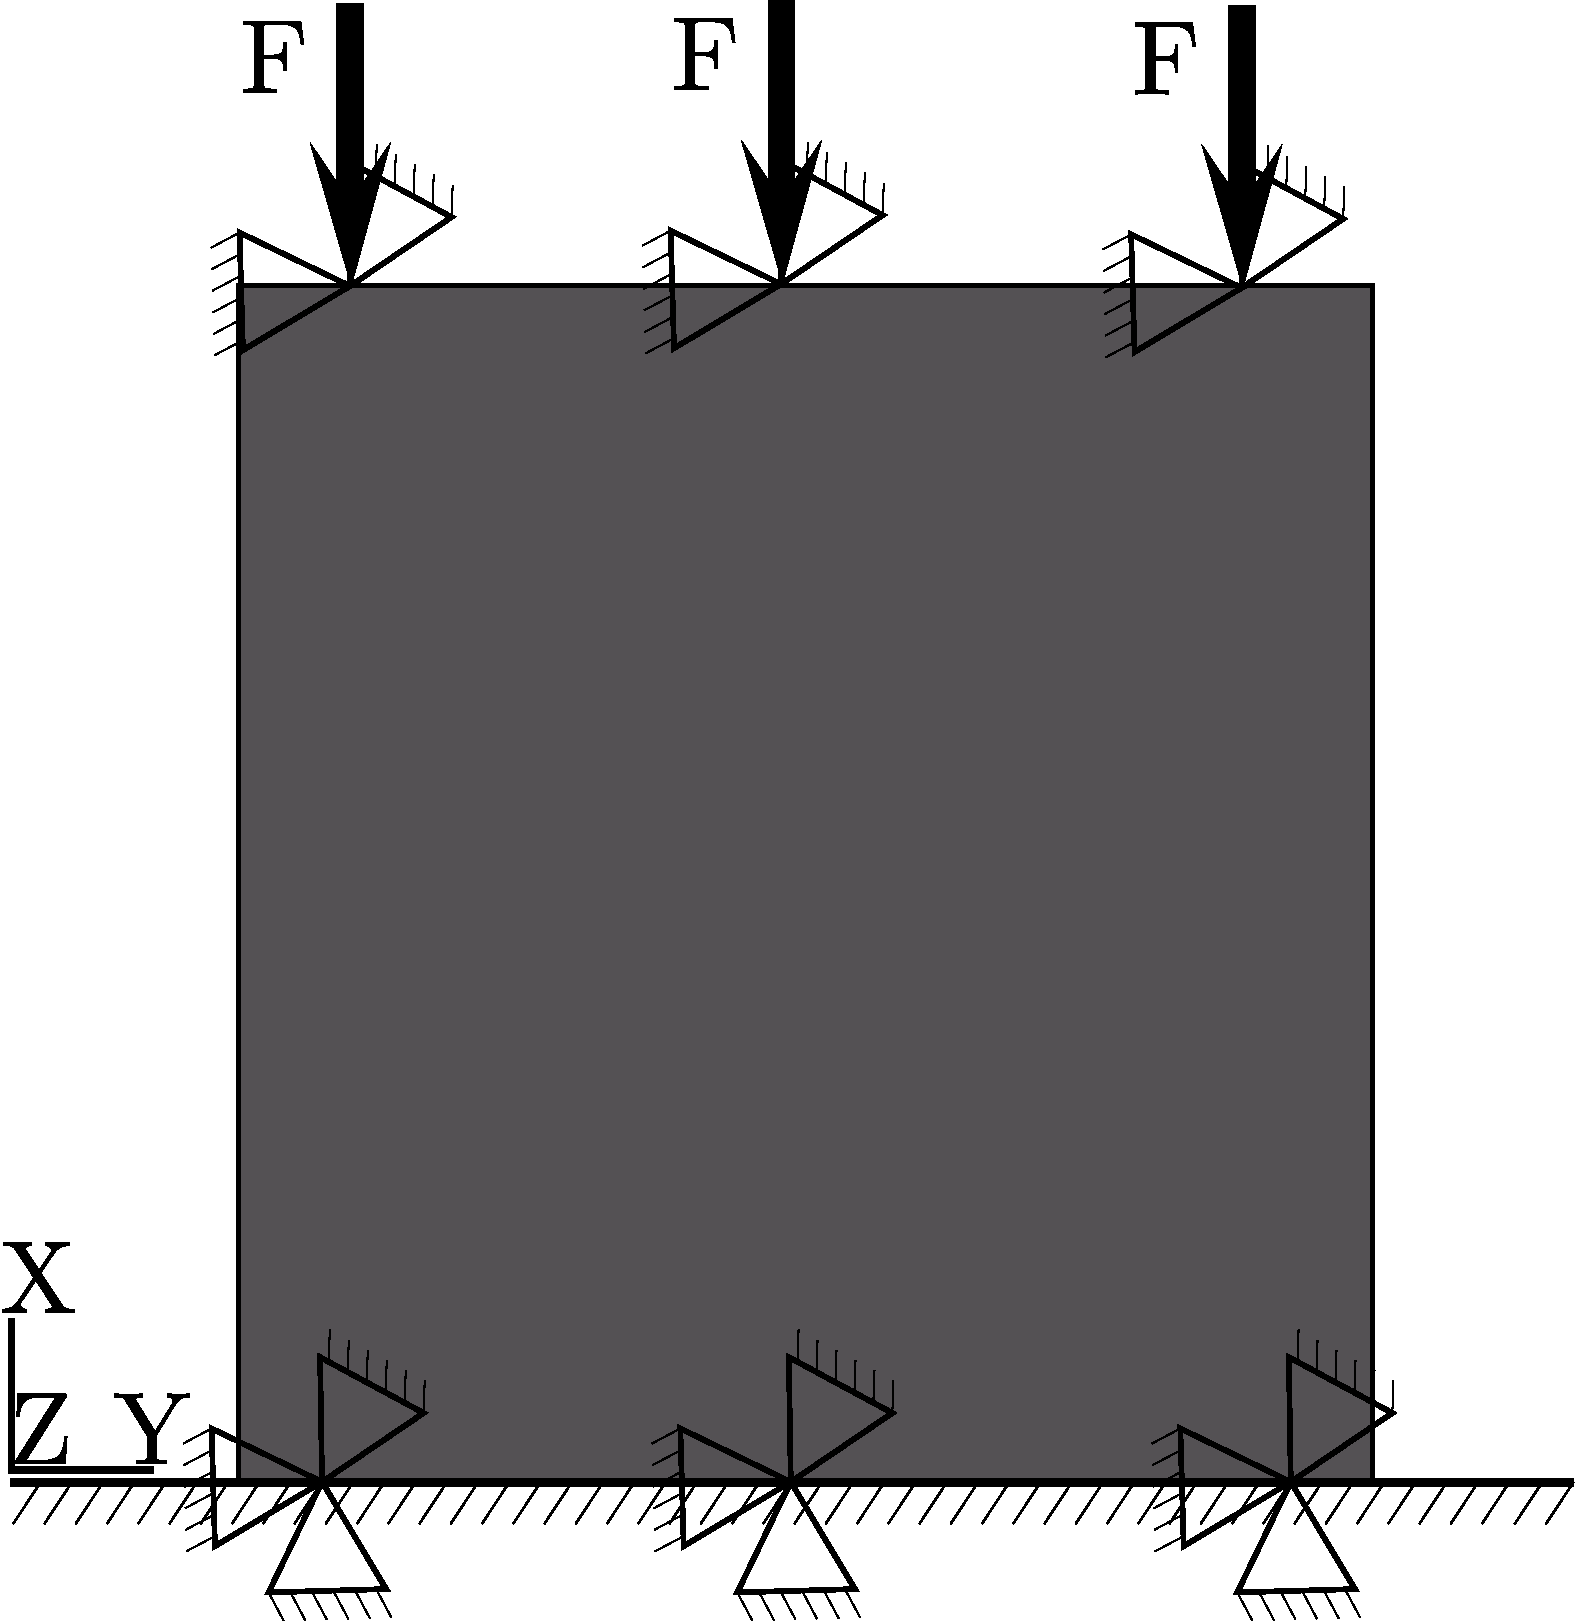
\includegraphics[width=\textwidth]{SIMPLE_MESH_F_1}
		\caption{}
	\end{subfigure}
	\caption{(a) Sample pore extracted by DN-RSA, and (b) the boundary conditions used in the simulations.}\label{stress_boundary}
\end{figure}
In \cite {heinzeExperimentalNumericalInvestigation2018}, 5 sample pores were extracted from an open foam sample with an average size of each pore  around $ 6 \times 6 \times 6 $ mm$ ^3 $. These were subjected to a compression test with the force-displacement response recorded. These samples were poured in Wood's metal to restrict strut movement and rotation as the samples were very small.

Since the samples being tested in the literature are from the same manufacturer as in \cite{jungMicrostructuralCharacterisationExperimental2017}, some sample single pores have been extracted from an RVE, and is scaled such that the average pore length for a 20 ppi foam is achieved. To mimic the compression test, the bottom faces along the preferential anisotropy direction in the samples are restricted in all directions. The top faces are restricted along the directions perpendicular to the loading direction (Figure \ref{stress_boundary}).


In Figure \ref{force_disp}, sample pore geometries taken from the RVE have been subjected to a uniaxial compression test. The yellow band represents the numerical observations of similar pore structures, as described in \cite{heinzeExperimentalNumericalInvestigation2018}. It can be seen that the Young modulus obtained for the sample pores are comparable to the simulated values of those modeled based on CT-scans of single pore structures in \cite{heinzeExperimentalNumericalInvestigation2018}. The variations in the pore geometries can explain the slightly high variations for the plastic collapse stress, or the plateau region of the plots.

\begin{figure}
	\centering
	\begin{subfigure}[b]{0.45\textwidth}
		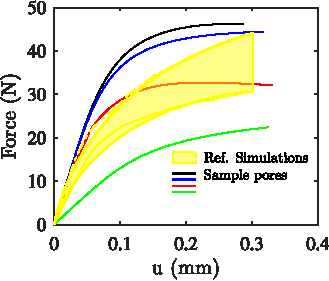
\includegraphics[width=\textwidth]{mini_pore_sim_1}
		\caption{}
	\end{subfigure}\\
	\begin{subfigure}[b]{0.33\textwidth}
		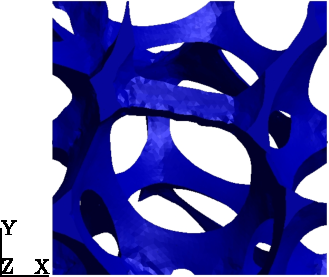
\includegraphics[width=\textwidth]{disp_pore_0}
		\caption{}
	\end{subfigure}
	\begin{subfigure}[b]{0.28\textwidth}
		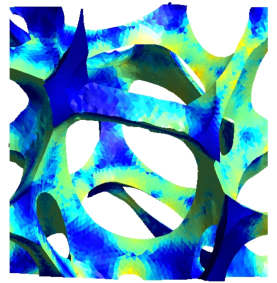
\includegraphics[width=\textwidth]{disp_pore_5}
		\caption{}
	\end{subfigure}
	\begin{subfigure}[b]{0.35\textwidth}
		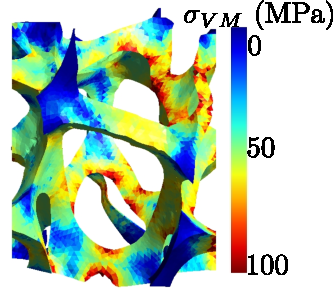
\includegraphics[width=\textwidth]{disp_pore_7}
		\caption{}
\end{subfigure}
	\caption{(a) Comparison of a simulation on a sample single pore generated in the RVE with the average maximum and minimum values in a force displacement plot of a similarly sized pore in \cite{heinzeExperimentalNumericalInvestigation2018}. (b)-(d) Shows the variation of the von Mises stress [MPa] in the micro-cell with the progress in the simulation of compression test on a single pore. 
%		TODO: Update plot with more realizations
	}\label{force_disp}
\end{figure}


\subsubsection*{RVE simulations}

\begin{figure}
	\centering
	\begin{subfigure}[b]{0.33\textwidth}
		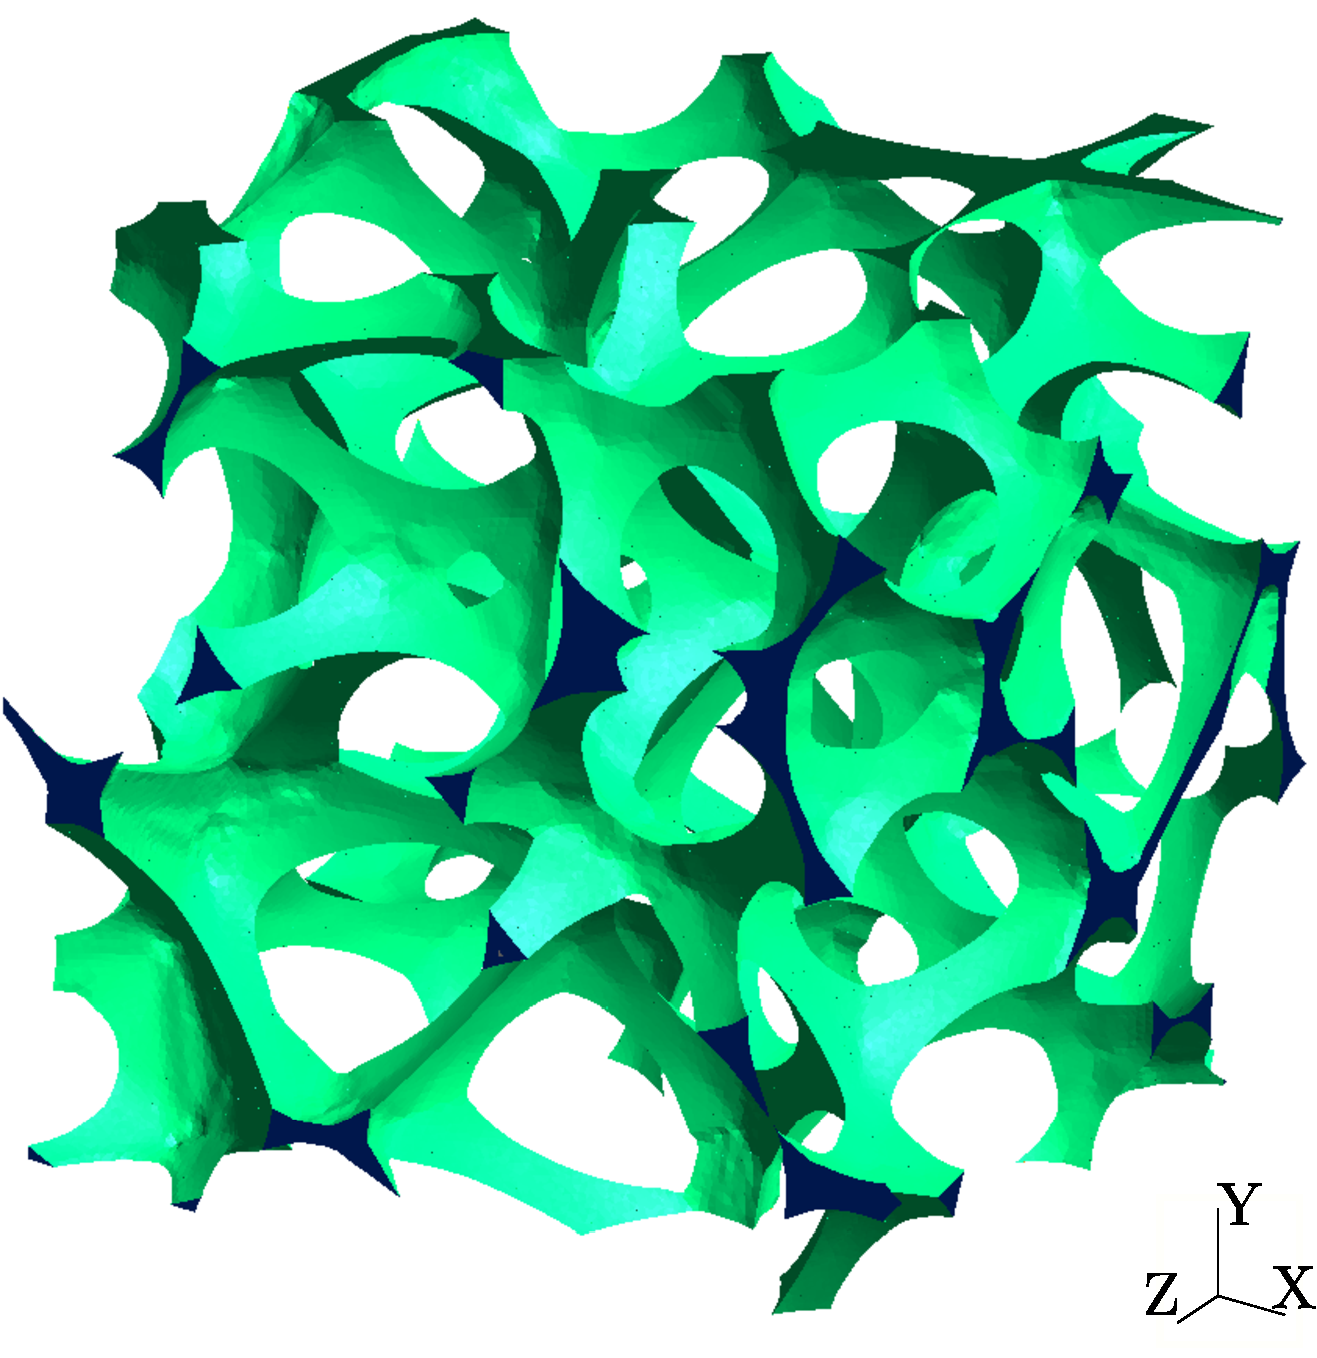
\includegraphics[width=\textwidth]{25_MESH}
		\caption{}
	\end{subfigure}
	\begin{subfigure}[b]{0.33\textwidth}
		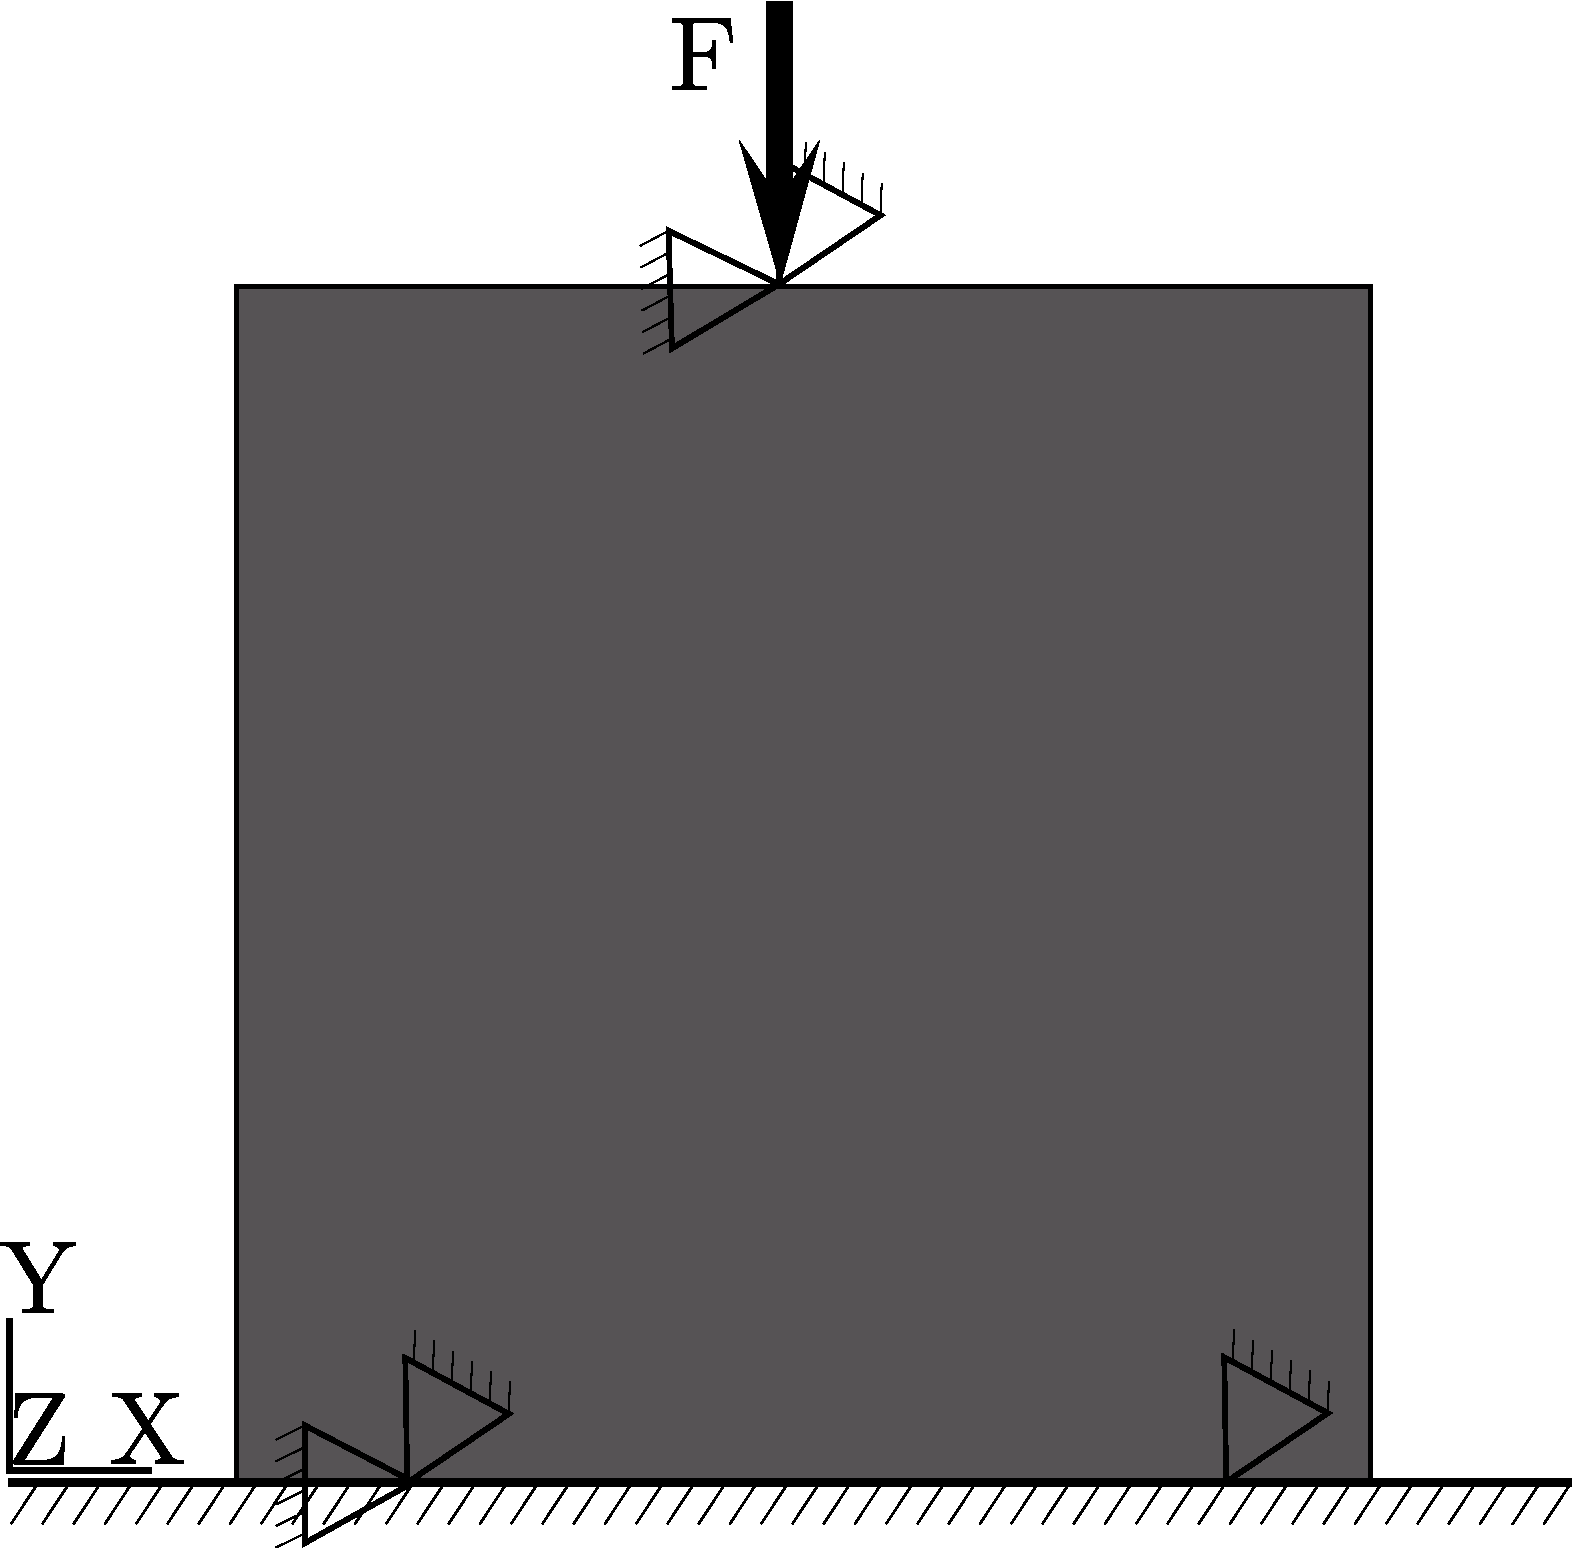
\includegraphics[width=\textwidth]{SIMPLE_MESH_f}
		\caption{}
	\end{subfigure}
	\caption{(a) An RVE generated using DN-RSA packing with an initial 100 pores resulting in 25 pores completely inside the RVE boundary after minus-sampling. (b) The boundary conditions imposed on the RVE for the finite element analysis. }\label{25_mesh}
\end{figure}

\begin{figure}
	\centering
	\begin{subfigure}[b]{0.45\textwidth}
		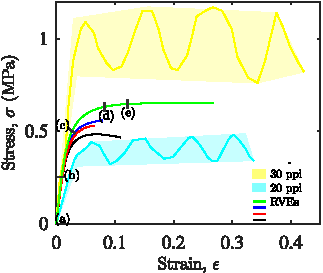
\includegraphics[width=\textwidth]{RVE_sim_1}
	\end{subfigure}
	\caption{Stress-strain diagram of the simulated RVE generated using DN-RSA packing in comparison with the values for 20 ppi and 30 ppi taken from \cite{jungMicrostructuralCharacterisationExperimental2017}. Markers (a)-(e) indicate the respective positions in Figure (\ref{25-stress-strain-2}). 
		%	TODO - Update plot with anne-jung data, update 4 more samples
	}\label{25-stress-strain}
\end{figure}

\begin{figure}
	\centering
	\begin{subfigure}[b]{0.32\textwidth}
		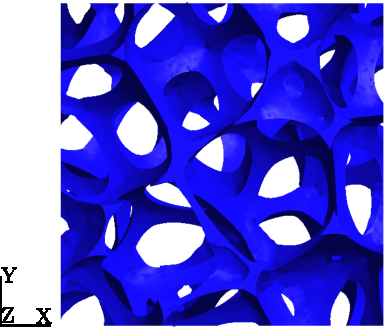
\includegraphics[width=\textwidth]{disp_fig_0}
		\caption{}
	\end{subfigure}
	\begin{subfigure}[b]{0.3\textwidth}
		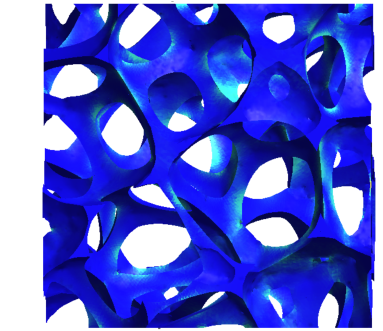
\includegraphics[width=\textwidth]{disp_fig_5}
		\caption{}
	\end{subfigure}\\
	\begin{subfigure}[b]{0.3\textwidth}
		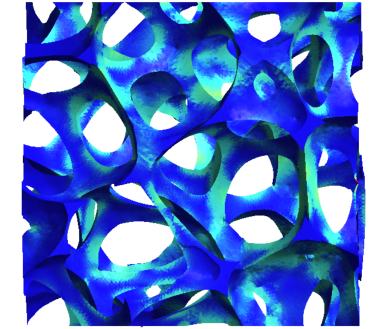
\includegraphics[width=\textwidth]{disp_fig_10}
		\caption{}
	\end{subfigure}
	\begin{subfigure}[b]{0.3\textwidth}
		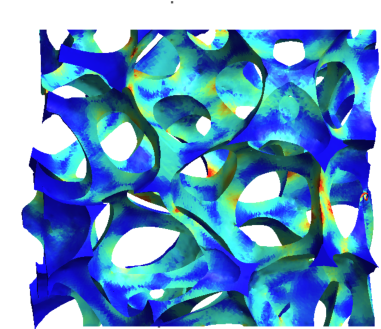
\includegraphics[width=\textwidth]{disp_fig_15}
		\caption{}
	\end{subfigure}
	\begin{subfigure}[b]{0.35\textwidth}
		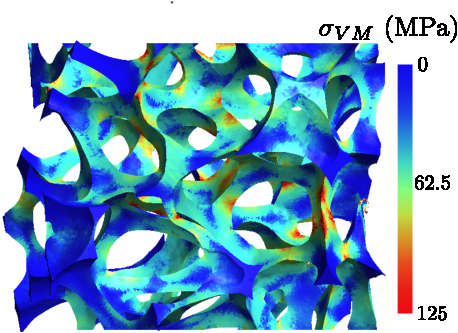
\includegraphics[width=\textwidth]{disp_fig_17}
		\caption{}
	\end{subfigure}
	\caption{(a)-(e) displays of the behavior of an RVE with 25 pores under uniaxial compression test. The von Mises stress is plotted on the deformed RVE.}\label{25-stress-strain-2}
\end{figure}
In a second set of simulations, entire RVEs with around 25 pores (Figure \ref{25_mesh}(a)) are subjected to a uniaxial compression test similar to that studied in \cite{jungMicrostructuralCharacterisationExperimental2017}. Figure \ref{25_mesh}(b) illustrates the boundary conditions used in the simulation that mimic the setting used in \cite{jungMicrostructuralCharacterisationExperimental2017}. The larger sample size means that  no special treatments was considered at the boundaries in the experimental setup, and thus, similar boundary conditions are imposed on the generated RVE.
{We, however, note that in order to simulate in an accurate way the experimental test performed on a foam sample having thousands of pores, a multiscale simulation would be required in order to properly represent the boundary conditions and the buckling behavior which occurs layer by layer. The simulation results should thus be seen as illustration of the possibility for the generated foam micro-structure to be used in a finite-element framework.} The effect of different BCs will be discussed in Section \ref{res-ct-fem}.

The RVEs here were generated to mimic the properties of a 20 ppi foam. The stress-strain diagram (Figure \ref{25-stress-strain}) shows that the curves are very close to the results of the 20 ppi foam taken from \cite{jungMicrostructuralCharacterisationExperimental2017} and similar properties can be observed for multiple RVEs with very small geometrical variations.
% Remarks Details possibly explained with more samples ** Statistics, boundary effect, more samples necessaryfox
It is to be noted that the criterion to enable a simulation with contact conditions was not used here due to the complexity of the geometry. This will need further investigation where the random geometry and the specific point of contact during the plastic failure is established. The deformation of a sample RVE is shown in Figure \ref{25-stress-strain-2} with the von Mises stress plotted on the deformed RVE.



\subsection{RVE obtained using DN-CT-SCAN with polyhedral packing from CT-scans}\label{res-ct-fem}

\begin{figure}
	\centering
	\begin{subfigure}{0.49\textwidth}
		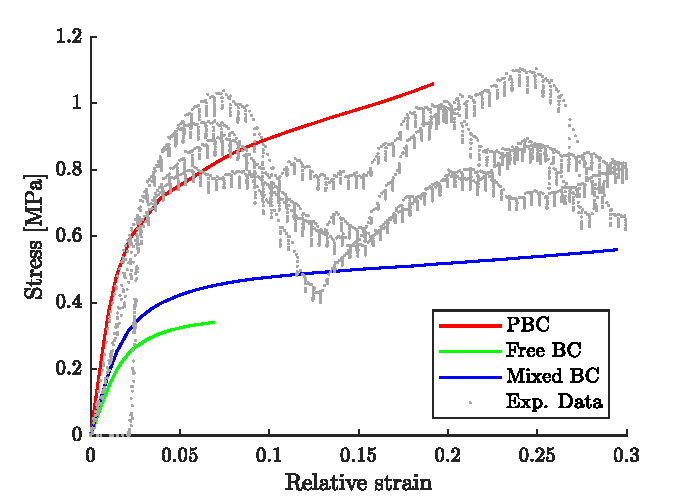
\includegraphics[width=\textwidth]{polyhedra_basis_compare}
	\end{subfigure}
	\begin{subfigure}{0.49\textwidth}
		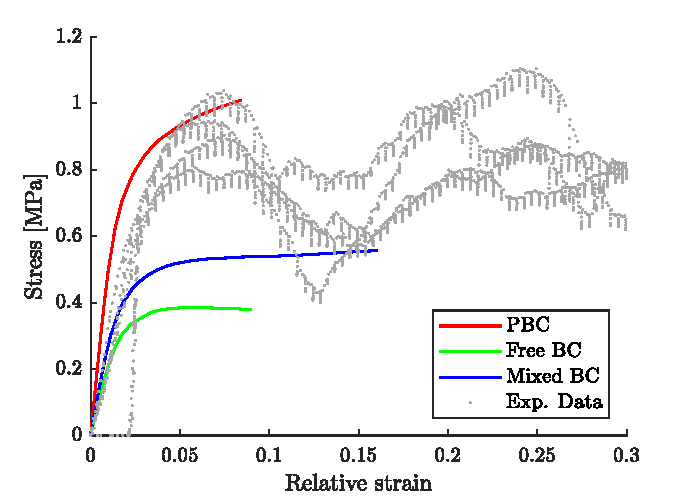
\includegraphics[width=\textwidth]{ellipsoid_basis_compare}
	\end{subfigure}
	\caption{Behavioral effect of various BCs on the micro-structure extracted using DN-CT-SCAN with (a) basis polyhedras and (b) basis ellipsoids, in comparison with experimental data as observed in \cite{jungMicrostructuralCharacterisationExperimental2017}. PBC is imposed using a 5th order Lagrangian polynomial based interpolation, free BC is uniaxial compression, and mixed BC signifies uniaxial compression with additional in-plane motion restrictions on the bounded box.}\label{fig-compare-polyelli}
\end{figure}


\begin{figure}
	\centering
	\begin{subfigure}[b]{0.42\textwidth}
		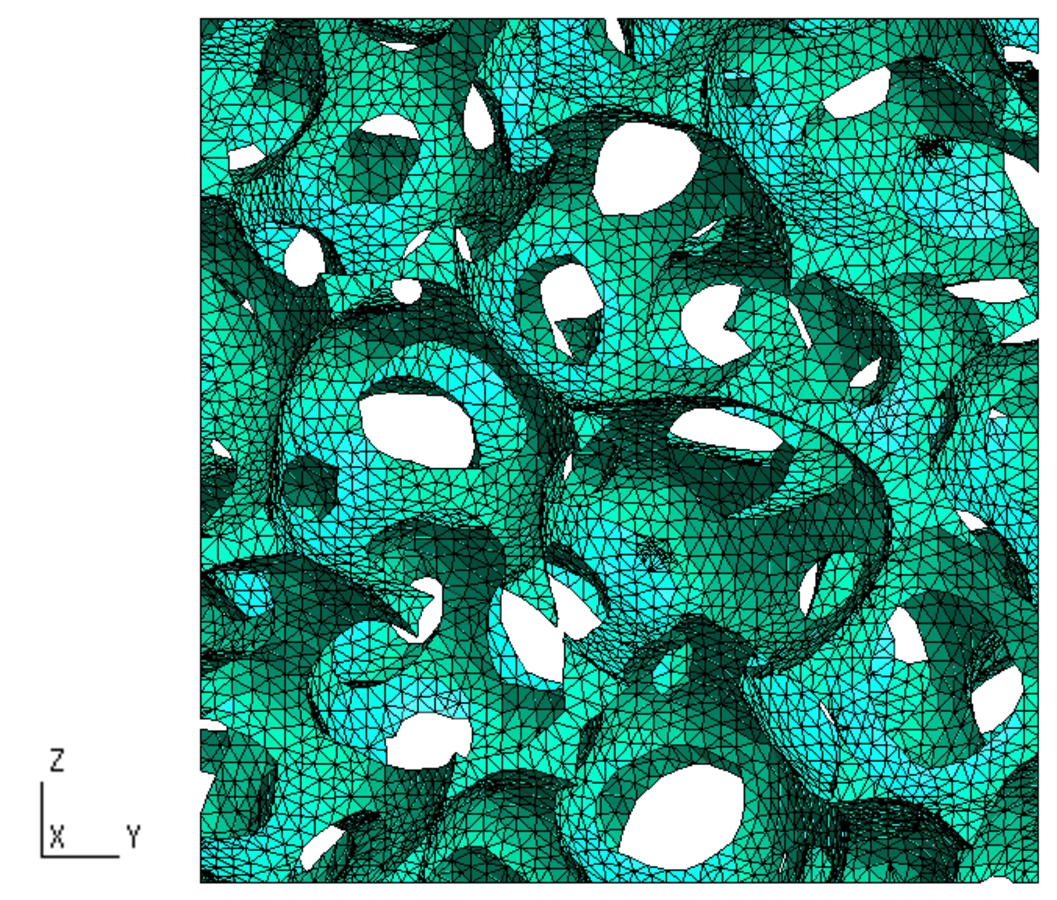
\includegraphics[width=\textwidth]{polyhedra_none}
		\caption{}
	\end{subfigure}
	\begin{subfigure}[b]{0.43\textwidth}
		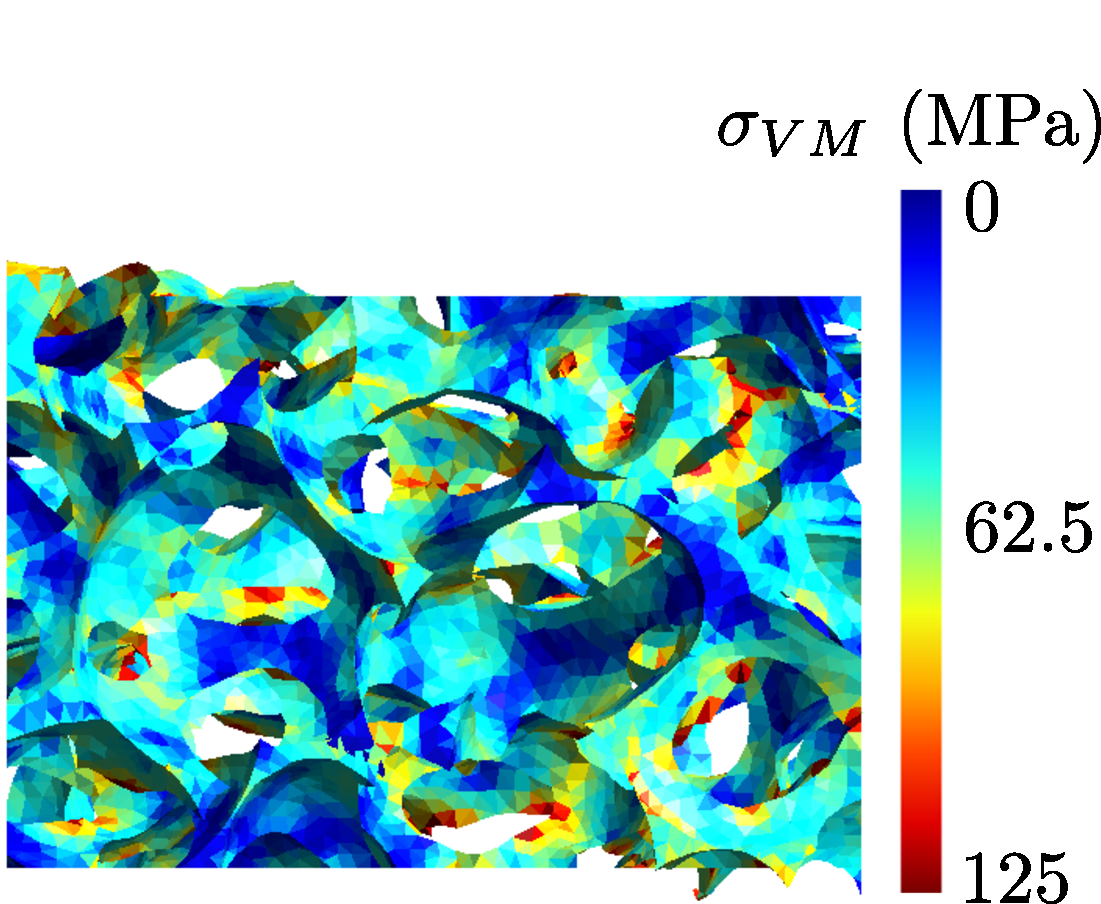
\includegraphics[width=\textwidth]{polyhedra_53}
		\caption{}
	\end{subfigure}
	\caption{(a) Finite element mesh of the morphology obtained from basis polyhedras using DN-CT-SCAN. (b) Behavior of the morphology under mixed BC uniaxial compression test at the moment of failure of convergence (corresponding to the final point of the Mixed BC curve in Figure \ref{fig-compare-polyelli}(a)). The von Mises stress is plotted on the deformed RVE.}\label{fig-snapshot-polyhedra-mbc}
\end{figure}

\begin{figure}
	\centering
	\begin{subfigure}{0.49\textwidth}
		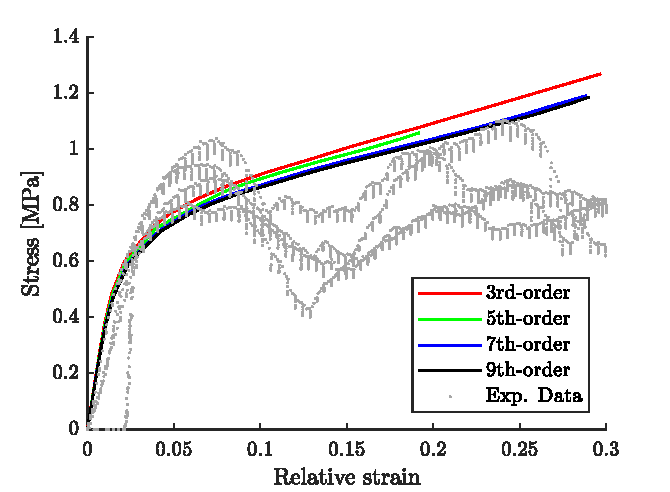
\includegraphics[width=\textwidth]{Polyhedra_PBC_polynomial_comparison_lagrange}
		\caption{}
	\end{subfigure}
	\begin{subfigure}{0.49\textwidth}
		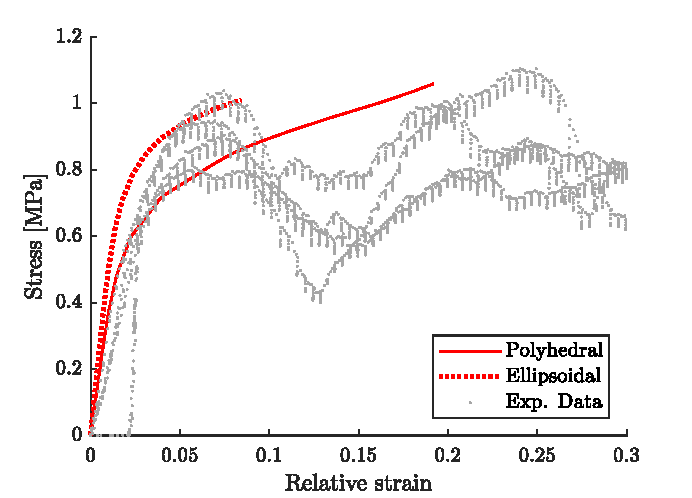
\includegraphics[width=\textwidth]{pbc_ellipsoid_polyhedra_compare}
		\caption{}
	\end{subfigure}
	\caption{(a) Behavioral effect of varying the order of polynomials used to impose PBC on the micro-structure using Lagrange interpolation method on comparison with experimental data as observed in \cite{jungMicrostructuralCharacterisationExperimental2017}. The micro-structure used here is extracted using DN-CT-SCAN using polyhedrals. (b) Difference in behavior of micro-structures depending on the basis used to construct the geometry from a given CT-Scan.}\label{fig-compare-pbc}
\end{figure}

Continuing on from Section \ref{res-ct}, the RVEs extracted using CT-scan based packing with DN-CT-SCAN are studied numerically. This study is an extension of the numerical study presented in Section \ref{res-fem-rsa} where the RVEs presented were randomly generated. The same material parameters are applied in this section also. 

Figure \ref{fig-compare-polyelli} presents the results for two RVEs, one based on the packing generated using the basis ellipsoids and the other using the basis polyhedrals. To understand the numerical behavior of the RVEs, various boundary conditions have been tested. The periodic boundary condition has been imposed using a 5th-order Lagrangian polynomial based interpolation method to enforce the periodicity of the boundary conditions as explained in \cite{nguyenImposingPeriodicBoundary2012}. The free boundary condition is nothing but uniaxial compression as described in Figure \ref{25_mesh}. The mixed boundary condition is attained by imposing a uniaxial load while ensuring that the bounding boxes deform along the normal perpendicular to the plane. Continuing on the morphological quantification analysis presented in Section \ref{res-ct}, the study of the numerical behavior shows that the polyhedrals packing based RVE is a much better choice than the ellipsoids packing based RVE (see Figure \ref{fig-compare-pbc}(b)) to continue the study of the behavior of open foams due to its better representation of the behavior during numerical simulations. A visual representation of the finite element mesh obtained using basis polyhedras is presented in Figure \ref{fig-compare-pbc}(a) and the deformation of this geometry under uniaxial compression with mixed BC is illustrated in Figure \ref{fig-compare-pbc}(b).

The imposition of various boundary conditions to study the behavior of the CT-scan based geometry is necessitated by the fact that the volume element extracted is in fact quite small compared to the random geometries extracted using DN-RSA. Such a study helps one obtain a general understanding of the impact smaller geometries can have on the overall homogenized behavior.

The application of various BC on the geometries warrants some observations regarding their applicability on a non-periodic geometry. The PBC condition adds extra constraints on the deformation of the struts and is not very realistic in this particular case due to the reduced size of the geometry along with its non-periodicity. This can be observed by the over-stiffness presented in the results. The mixed BC, in comparison, avoids the artificial constraints imposed on the strut deformation and exhibits a comparable stiffness as observed experimentally but displays plastic deformation quite early in the analysis. Finally, the free BC induce unrealistic deformations as compared to what can be expected in an embedded body, because it is very compliant and softens fast as compared to the other 2 BCs.

Figure \ref{fig-compare-pbc}(a) presents the dependency of the order of the polynomial used to impose the PBC with the Lagrange interpolation method. The convergence of the scheme can be observed on using higher order polynomials to the experimental values when tried with the micro-structure extracted using DN-CT-SCAN with polyhedral basis.

\section{Conclusions}
In this Chapter, geometries that have been randomly extracted using DN-RSA have been compared in detail with existing Laguerre tessellation-based models that show the geometrical resemblance of these random models. Various open foam morphological indicators like face-to-cell ratio, edge-to-face ratio, strut length distributions and strut cross-section variations have been quantified. This comparison has been extended to morphologies that have been reconstructed based on CT scans of physical samples to validate the use of the DN-RSA tool as a morphology reconstructing tool. 

A numerical study on sample individual pores constituting the larger RVE using established parameters from other studies has been presented that show the numerical behavior to be very similar to the behavior of actual pores. As an expansion of this study, uniaxial compression tests of sample RVEs using material parameters established in literature shows the similarities in the mechanical properties of the RVEs to that of open foam material having a similar pore structure. A similar numerical study has been conducted on reconstructed morphologies, and a comparison has been conducted on geometries extracted using the basis ellipsoids and the basis polyhedrals under various boundary conditions. The results have been found to be very close to the experimental data, especially for the geometries extracted using basis polyhedrals, establishing the benefits of the use of extracting accurate geometry to represent complex micro-structures like those of open foam materials.

A study on the overall impact of various boundary conditions, especially on small geometries has been presented by using periodic boundary conditions, free boundary condition and an intermediate boundary condition that tries to reduce the constraints imposed by PBC while ensuring that the struts of small geometries do not behave in an unexpectedly compliant manner.